\thispagestyle{toancuabinone}
\pagestyle{toancuabi}
\everymath{\color{toancuabi}}
\graphicspath{{../toancuabi/pic/}}
\begingroup
\AddToShipoutPicture*{\put(0,616){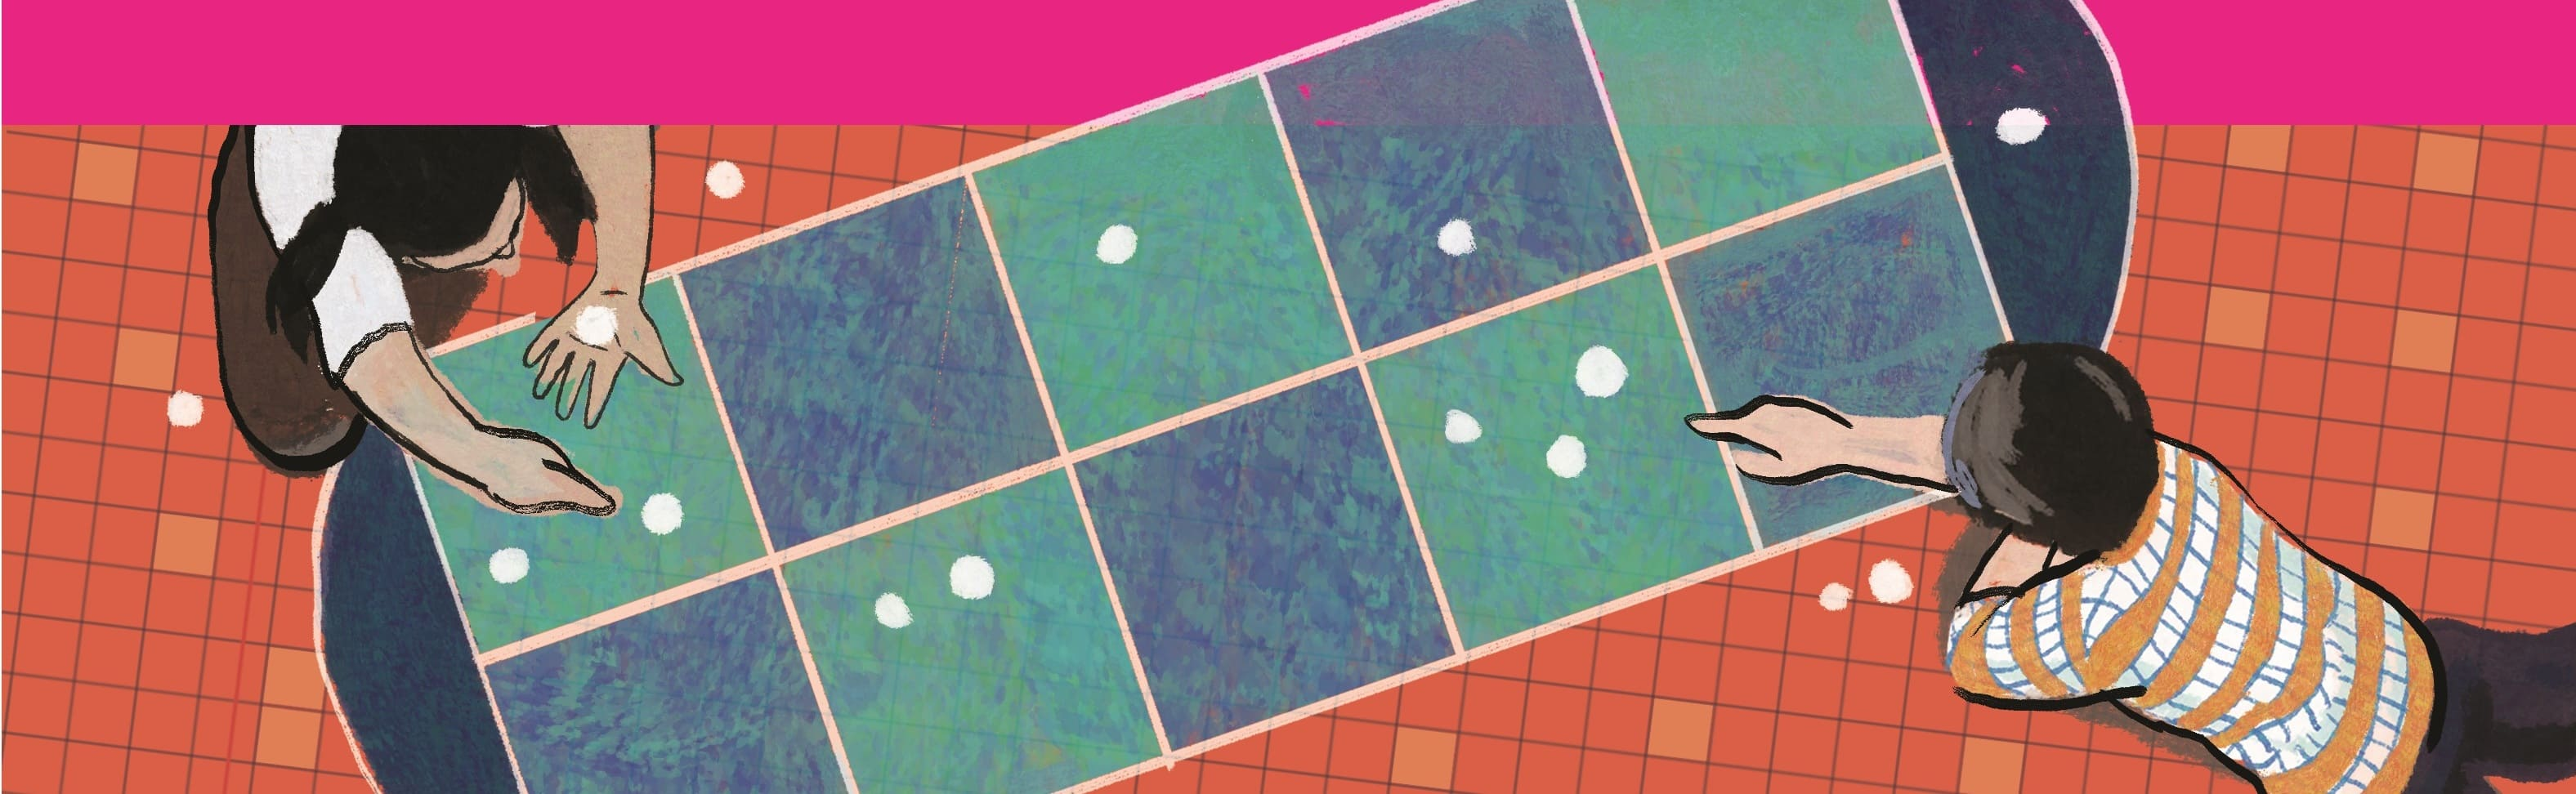
\includegraphics[width=19.3cm]{../bannertoancuabi}}}  
\AddToShipoutPicture*{\put(66,492){
\includegraphics[scale=1]{../tieude1.pdf}}} 
\centering
\endgroup
\vspace*{215pt}

\begin{multicols}{2}
Mở rộng bài toán số $5$, các bạn thử sức của mình xem sao nhé.
\vskip 0.1cm
	\textbf{\color{toancuabi}Bài toán $\pmb{6.1}$ (Apmops)}
	\vskip 0.1cm
	Cho các điểm $A1$, $A2$, $A3$, $B1$, $B2$, $B3$, $B4$, $C1$, $C2$, $C3$, $C4$ và $C5$ nằm trên $3$ đường thẳng như hình vẽ. Có bao nhiêu tam giác được tạo bởi $3$ trong các đỉnh đã cho?
	\begin{figure}[H]
			\centering
			\vspace*{-5pt}
			\captionsetup{labelformat=empty, justification=centering}
			\begin{tikzpicture}[toancuabi, scale=0.9]
					\draw  (-5.4,1.6)-- (-1.7,5.32);
					\draw  (-2.74,5.5)-- (0.28,1.64);
					\draw  (-5.6,2.)-- (0.78,2.02);
					\draw[fill=white]  (-4.45248688627018,2.552634806236469) circle (1.5pt);
					\draw (-4.61,3.02) node {$A_1$};
					\draw[fill=white]  (-3.6547027796748095,3.3547312593539766) circle (1.5pt);
					\draw (-3.91,3.88) node {$A_2$};
					\draw[fill=white]  (-2.856811147760132,4.1569358190087335) circle (1.5pt);
					\draw (-3.09,4.66) node {$A_3$};
					\draw[fill=white]  (-1.8796143213988348,4.400301748542881) circle (1.5pt);
					\draw (-1.69,4.82) node {$B_1$};
					\draw[fill=white]  (-1.4504776019983348,3.851802497918401) circle (1.5pt);
					\draw (-1.27,4.28) node {$B_2$};
					\draw[fill=white]  (-0.9673278934221485,3.2342667776852623) circle (1.5pt);
					\draw (-0.77,3.66) node {$B_3$};
					\draw[fill=white]  (-0.5014784346378021,2.6388432972522895) circle (1.5pt);
					\draw (-0.31,3.06) node {$B_4$};
					\draw[fill=white]  (-4.359949489986439,2.003887305674024) circle (1.5pt);
					\draw (-4.43,1.5) node {$C_1$};
					\draw [fill=white] (-3.619831371238773,2.0062074251685305) circle (1.5pt);
					\draw (-3.63,1.5) node {$C_2$};
					\draw[fill=white]  (-2.0000353766631944,2.0112851555590496) circle (1.5pt);
					\draw (-2.03,1.5) node {$C_3$};
					\draw[fill=white]  (-1.3800414693107446,2.0132287101275526) circle (1.5pt);
					\draw (-1.43,1.5) node {$C_4$};
					\draw[fill=white]  (-0.839921385192901,2.0149218765354453) circle (1.5pt);
					\draw (-0.77,1.5) node {$C_5$};
				\end{tikzpicture}
			\vspace*{-15pt}
		\end{figure}
	\textbf{\color{toancuabi}Bài toán $\pmb{6.2}$}
	Có bao nhiêu tam giác trong hình vẽ?
	\begin{figure}[H]
			\centering
			\vspace*{-10pt}
			\captionsetup{labelformat=empty, justification=centering}
			\begin{tikzpicture}[toancuabi,scale=0.9]
					\draw  (1.,3.)-- (-1.44,0.);
					\draw  (-1.44,0.)-- (4.,0.);
					\draw  (4.,0.)-- (1.,3.);
					\draw  (1.,3.)-- (0.,0.);
					\draw  (1.,3.)-- (1.4,0.);
					\draw  (1.,3.)-- (2.68,0.);
					\draw  (4.,0.)-- (0.,1.7704918032786887);
					\draw  (-1.44,0.)-- (2.,2.);
					\draw  (-1.44,0.)-- (3.37,0.63);
						\draw [fill=white] (1.,3.) circle (1.5pt);
						\draw [fill=white] (-1.44,0.) circle (1.5pt);
						\draw [fill=white] (4.,0.) circle (1.5pt);
						\draw [fill=white] (0.,0.) circle (1.5pt);
						\draw [fill=white] (1.4,0.) circle (1.5pt);
						\draw [fill=white] (2.68,0.) circle (1.5pt);
						\draw [fill=white] (0.,1.7704918032786887) circle (1.5pt);
						\draw [fill=white] (2.,2.) circle (1.5pt);
						\draw [fill=white] (3.37,0.63) circle (1.5pt);
				\end{tikzpicture}
			\vspace*{-5pt}
		\end{figure}
	\textbf{\color{toancuabi}Bài toán $\pmb{6.3}$}
	Có bao nhiêu tam giác được tạo bởi $3$ trong $12$ điểm đã cho trên lưới ô vuông như hình vẽ?
	\begin{figure}[H]
			\centering
			\vspace*{
				5pt}
			\captionsetup{labelformat=empty, justification=centering}
			\begin{tikzpicture}[toancuabi,scale=0.7]
					\draw [xstep=1.0cm,ystep=1.0cm] (-2.78,-0.8) grid (4.82,4.78);
						\draw [fill=cackithi!40] (-2.,4.) circle (5.0pt);
						\draw [fill=cackithi!40] (0.,4.) circle (5.0pt);
						\draw [fill=cackithi!40] (2.,4.) circle (5.0pt);
						\draw [fill=cackithi!40] (4.,4.) circle (5.0pt);
						\draw [fill=cackithi!40] (4.,2.) circle (5.0pt);
						\draw [fill=cackithi!40] (4.,0.) circle (5.0pt);
						\draw [fill=cackithi!40] (2.,0.) circle (5.0pt);
						\draw [fill=cackithi!40] (2.,2.) circle (5.0pt);
						\draw [fill=cackithi!40] (0.,2.) circle (5.0pt);
						\draw [fill=cackithi!40] (0.,0.) circle (5.0pt);
						\draw [fill=cackithi!40] (-2.,2.) circle (5.0pt);
						\draw [fill=cackithi!40] (-2.,0.) circle (5.0pt);
				\end{tikzpicture}
			\vspace*{-5pt}
		\end{figure}
\textbf{\color{toancuabi}Bài toán số $\pmb{7}$: (Apmops)}
\vskip 0.1cm
Có bao nhiêu cách để tô $6$ mặt của một hình lập phương bằng $6$ mầu, mỗi mặt được tô bằng $1$ mầu sao cho không có hai mặt nào có cùng mầu? (Hai cách tô mầu được coi là như nhau nếu chúng nhìn giống hệt nhau sau một phép xoay hình). 
\vskip 0.1cm
\textbf{\color{toancuabi}Phân tích bài toán:} Hướng đi thứ nhất, ta hình dung nếu cố định hình lập phương lại và mỗi cách nhìn khác nhau ở mỗi phía được coi là khác nhau, như thế thì số cách tô sẽ như tô theo hàng ngang ($6$ người ngồi trên $6$ cái ghế trên $1$ hàng) và sẽ là $6!=720$ cách. Do hình lập phương này xoay được nên ta xem mỗi một kiểu tô có bao nhiêu cách xoay nó xung quanh chính nó. Do có $6$ mầu ta có $6$ cách xoay để có đáy khác mầu. Mỗi cách đặt đáy với $1$ mầu ta có $4$ cách xoay xung quanh chính nó (do hình lập phương có $4$ cạnh bên), từ đó ta có hướng giải quyết bài toán.
\vskip 0.1cm
Hướng đi thứ $2$, do hình lập phương xoay được nên ta có thể cố định mầu ở những vị trí ta có thể xoay nó về và ta sẽ có hướng giải quyết bài toán như lời giải $2$.
\vskip 0.1cm
Hướng đi thứ $3$ gần giống với hướng thứ $2$, ta có thể hình dung mình có thể tô mầu ở đáy bằng mầu tùy thích do hình lập phương xoay được, mặt đối diện trên đỉnh sẽ còn $5$ cách tô, $4$ mặt xung quanh ta sẽ hình dung nó như $4$ người ngồi xung quanh một cái bàn tròn nên ta có thể áp dụng bài toán hoán vị vòng tròn để giải quyết.
\vskip 0.1cm
\textit{Lời giải $1$:}
Giả sử hình lập phương cố định, khi đó ta có $6!=720$ cách tô.
\vskip 0.1cm
Mỗi cách tô ta có $6$ cách đặt các mặt khác mầu nhau xuống đáy, khi đặt rồi ta có $4$ cách xoay xung quanh nó, vậy ứng với mỗi cách tô mầu ta có $6\times4=24$ cách xoay nó xung quanh chính nó. Vậy số cách tô mầu là: $720:24=30$ (cách).
\vskip 0.1cm
\textit{Lời giải $2$:}
Đầu tiên ta tô mầu $1$ mặt (mầu ta thích), rồi đặt nó xuống đáy, khi đó ở mặt đối diện trên đỉnh có $5$ cách tô.
\vskip 0.1cm
Tiếp theo ta tô mầu $1$ mặt xung quanh (mầu ta thích trong $4$ mầu còn lại), rồi xoay nó sang bên trái, khi đó mặt bên phải có $3$ cách tô, còn $2$ mặt còn lại (trước và sau) có $2!$ cách tô, vậy số cách tô mầu là: $1\times5\times1\times3\times2!=30$ (cách)
\vskip 0.1cm
\textit{Lời giải $3$:}
Tương tự như lời giải $2$, đầu tiên ta tô mầu $1$ mặt (mầu ta thích), rồi đặt nó xuống đáy, khi đó ở mặt đối diện trên đỉnh có $5$ cách tô.
\vskip 0.1cm
Còn $4$ mặt xung quanh, do xoay được nên theo bài toán hoán vị vòng tròn ta có $4!/4=6$ cách tô.
\vskip 0.1cm
Vậy số cách tô mầu hình lập phương là: $5\times 6=30$ (cách).
\vskip 0.1cm
\textbf{\color{toancuabi}Bài toán số $\pmb{8}$: (IMSO)}
\vskip 0.1cm
Một hình lập phương được tô các mặt bằng $6$ mầu, mỗi mặt $1$ mầu khác nhau và được đánh số từ $1$ đến $6$ sao cho tổng hai mặt đối diện bằng $7$. Hỏi có bao nhiêu cách tô mầu và đánh số hình lập phương này? (Hai cách tô mầu, đánh số được coi là như nhau nếu chúng nhìn giống hệt nhau sau một phép xoay hình). 
\vskip 0.1cm
Phân tích bài toán: Bài toán này là tương đối khó khi các bạn lớp $5,6$ đi thi gặp phải, và đúng là trong năm thi đó đoàn học sinh Việt Nam chỉ có đúng $1$ bạn làm được, tuy nhiên nếu chia bài toán làm hai bước, bước $1$ tô mầu, bước $2$ điền số thì ta có thể giải quyết được bài toán một cách tương đối dễ dàng.
\vskip 0.1cm
\textit{Lời giải:}
Bước $1$: Tô mầu hình lập phương, theo bài toán số $7$, ta có $30$ cách tô mầu hình lập phương này.
\vskip 0.1cm
Bước $2$: Đánh số, ta đánh theo thứ tự:
\vskip 0.1cm
Đánh số $1$, có $6$ cách. Đánh số $6$ ở mặt đối diện số $1$, có $1$ cách.
\vskip 0.1cm
Đánh số $2$, có $4$ cách (do còn $4$ mặt chưa đánh số). Đánh số $5$ ở mặt đối diện, có $1$ cách.
\vskip 0.1cm
Đánh số $3$, có $2$ cách (do còn $2$ mặt chưa đánh số). Đánh số $4$ ở mặt đối diện, có $1$ cách.
\vskip 0.1cm
Vậy ta có $6\times1\times4\times1\times2\times1=48$ cách đánh số.
\vskip 0.1cm
Theo quy tắc nhân ta có số cách tô mầu và đánh số là: $30\times 48=1440$ (cách).
\vskip 0.1cm
\textbf{\color{toancuabi}Bài toán số $\pmb{9}$: (IMAS)}
\vskip 0.1cm
	Một bàn cờ hình vuông $5\times 5$ được xếp một hình chữ L chiếm $4$ ô như hình vẽ. Ta có thể xoay hoặc lật hình chữ L này. Hỏi có bao nhiêu cách xếp hình chữ L này vào bàn cờ hình vuông đã cho?
	\begin{figure}[H]
			\centering
			\vspace*{-5pt}
			\captionsetup{labelformat=empty, justification=centering}
			\begin{tikzpicture}[toancuabi,scale=0.65]
					\filldraw[cackithi!40] (0,0) rectangle (1,3);
					\filldraw[cackithi!40] (1,0) rectangle (2,1);
					\draw (0,0) grid (5,5);
				\end{tikzpicture}
			\vspace*{-10pt}
		\end{figure}
\textbf{\color{toancuabi}Phân tích bài toán:} Ta nhận thấy hình chữ L tô đen có thể xoay hoặc lật được, nên ta sẽ xem nó có thể có bao nhiêu cách biến hình (xoay hoặc lật).  Ứng với mỗi phép biến hình bằng xoay, lật ta xem có bao nhiêu cách trượt nó theo hàng ngang và hàng dọc, từ đó ta có cách giải quyết bài toán.
\vskip 0.1cm
\textit{Lời giải:}
Ta tính số cách xoay, lật hình chữ L tô đậm, như hình dưới ta có $8$ cách.
\begin{figure}[H]
		\centering
		\vspace*{-5pt}
		\captionsetup{labelformat=empty, justification=centering}
		\begin{tikzpicture}[toancuabi,scale=0.385]
				\fill[cackithi!40] (1.,3.) -- (2.,3.) -- (2.,1.) -- (3.,1.) -- (3.,0.) -- (1.,0.) -- cycle;
				\fill[cackithi!40] (5.,0.) -- (7.,0.) -- (7.,3.) -- (6.,3.) -- (6.,1.) -- (5.,1.) -- cycle;
				\fill[cackithi!40] (9.,2.) -- (11.,2.) -- (11.,3.) -- (12.,3.) -- (12.,1.) -- (9.,1.) -- cycle;
				\fill[cackithi!40] (14.,3.) -- (14.,1.) -- (17.,1.) -- (17.,2.) -- (15.,2.) -- (15.,3.) -- cycle;
				\fill[cackithi!40] (3.,-2.) -- (1.,-2.) -- (1.,-5.) -- (2.,-5.) -- (2.,-3.) -- (3.,-3.) -- cycle;
				\fill[cackithi!40] (5.,-2.) -- (7.,-2.) -- (7.,-5.) -- (6.,-5.) -- (6.,-3.) -- (5.,-3.) -- cycle;
				\fill[cackithi!40] (9.,-2.) -- (12.,-2.) -- (12.,-4.) -- (11.,-4.) -- (11.,-3.) -- (9.,-3.) -- cycle;
				\fill[cackithi!40] (14.,-2.) -- (14.,-4.) -- (15.,-4.) -- (15.,-3.) -- (17.,-3.) -- (17.,-2.) -- cycle;
				\draw [] (1.,3.)-- (2.,3.);
				\draw [] (2.,3.)-- (2.,1.);
				\draw [] (2.,1.)-- (3.,1.);
				\draw [] (3.,1.)-- (3.,0.);
				\draw [] (3.,0.)-- (1.,0.);
				\draw [] (1.,0.)-- (1.,3.);
				\draw [] (5.,0.)-- (7.,0.);
				\draw [] (7.,0.)-- (7.,3.);
				\draw [] (7.,3.)-- (6.,3.);
				\draw [] (6.,3.)-- (6.,1.);
				\draw [] (6.,1.)-- (5.,1.);
				\draw [] (5.,1.)-- (5.,0.);
				\draw [] (9.,2.)-- (11.,2.);
				\draw [] (11.,2.)-- (11.,3.);
				\draw [] (11.,3.)-- (12.,3.);
				\draw [] (12.,3.)-- (12.,1.);
				\draw [] (12.,1.)-- (9.,1.);
				\draw [] (9.,1.)-- (9.,2.);
				\draw [] (14.,3.)-- (14.,1.);
				\draw [] (14.,1.)-- (17.,1.);
				\draw [] (17.,1.)-- (17.,2.);
				\draw [] (17.,2.)-- (15.,2.);
				\draw [] (15.,2.)-- (15.,3.);
				\draw [] (15.,3.)-- (14.,3.);
				\draw [] (3.,-2.)-- (1.,-2.);
				\draw [] (1.,-2.)-- (1.,-5.);
				\draw [] (1.,-5.)-- (2.,-5.);
				\draw [] (2.,-5.)-- (2.,-3.);
				\draw [] (2.,-3.)-- (3.,-3.);
				\draw [] (3.,-3.)-- (3.,-2.);
				\draw [] (5.,-2.)-- (7.,-2.);
				\draw [] (7.,-2.)-- (7.,-5.);
				\draw [] (7.,-5.)-- (6.,-5.);
				\draw [] (6.,-5.)-- (6.,-3.);
				\draw [] (6.,-3.)-- (5.,-3.);
				\draw [] (5.,-3.)-- (5.,-2.);
				\draw [] (9.,-2.)-- (12.,-2.);
				\draw [] (12.,-2.)-- (12.,-4.);
				\draw [] (12.,-4.)-- (11.,-4.);
				\draw [] (11.,-4.)-- (11.,-3.);
				\draw [] (11.,-3.)-- (9.,-3.);
				\draw [] (9.,-3.)-- (9.,-2.);
				\draw [] (14.,-2.)-- (14.,-4.);
				\draw [] (14.,-4.)-- (15.,-4.);
				\draw [] (15.,-4.)-- (15.,-3.);
				\draw [] (15.,-3.)-- (17.,-3.);
				\draw [] (17.,-3.)-- (17.,-2.);
				\draw [] (17.,-2.)-- (14.,-2.);
				\draw  (0.,4.)-- (18.,4.);
				\draw  (18.,4.)-- (18.,-6.);
				\draw  (18.,-6.)-- (0.,-6.);
				\draw  (0.,4.)-- (0.,-6.);
				\draw  (0.,-1.)-- (18.,-1.);
				\draw  (13.,4.)-- (13.,-6.);
				\draw  (8.,4.)-- (8.,-6.);
				\draw  (4.,4.)-- (4.,-6.);
				\draw  (1.,2.)-- (2.,2.);
				\draw  (1.,1.)-- (2.,1.);
				\draw  (2.,1.)-- (2.,0.);
				\draw  (6.,2.)-- (7.,2.);
				\draw  (6.,1.)-- (7.,1.);
				\draw  (6.,1.)-- (6.,0.);
				\draw  (11.,2.)-- (11.,1.);
				\draw  (10.,2.)-- (10.,1.);
				\draw  (11.,2.)-- (12.,2.);
				\draw  (15.,2.)-- (15.,1.);
				\draw  (15.,2.)-- (14.,2.);
				\draw  (16.,2.)-- (16.,1.);
				\draw  (15.,-2.)-- (15.,-3.);
				\draw  (16.,-2.)-- (16.,-3.);
				\draw  (15.,-3.)-- (14.,-3.);
				\draw  (11.,-3.)-- (12.,-3.);
				\draw  (11.,-3.)-- (11.,-2.);
				\draw  (10.,-2.)-- (10.,-3.);
				\draw  (6.,-3.)-- (7.,-3.);
				\draw  (7.,-4.)-- (6.,-4.);
				\draw  (6.,-3.)-- (6.,-2.);
				\draw  (2.,-3.)-- (2.,-2.);
				\draw  (2.,-3.)-- (1.,-3.);
				\draw  (1.,-4.)-- (2.,-4.);
			\end{tikzpicture}
		\vspace*{-10pt}
	\end{figure}
Ứng với mỗi cách biến hình này, ta xem có bao nhiêu cách dời hình theo hàng ngang và hàng dọc, và ta tính được số cách dời hình bằng trượt (tịnh tiến) theo hai chiều ngang, dọc là: $3\times4=12$.
\begin{figure}[H]
		\centering
		\vspace*{-10pt}
		\begin{tikzpicture}[toancuabi,scale=0.62, node font= \scriptsize]
				\filldraw[cackithi!40] (0,0) rectangle (1,3);
				\filldraw[cackithi!40] (1,0) rectangle (2,1);
				\draw (0,0) grid (5,5);
				\draw (1.5,0.5) node {$1$};
				\draw (2.5,0.5) node {$2$};
				\draw (3.5,0.5) node {$3$};
				\draw (4.5,0.5) node {$4$};
				\draw (0.5,2.5) node {$1$};
				\draw (0.5,3.5) node {$2$};
				\draw (0.5,4.5) node {$3$};			
				\draw (0.2, 5.5) node[right] {$3$ cách di chuyển theo cột dọc};
				\draw (5.2, 0.4) node[right] {$4$ cách di chuyển theo hàng ngang};
			\end{tikzpicture}
		\vspace*{-15pt}
	\end{figure}
	Theo quy tắc nhân, ta có số cách đặt chữ L vào ô vuông $5\times 5$ là: $8\times12=96$ (cách)
\vskip 0.1cm
Mở rộng bài toán số $9$. Các bạn thử sức mình xem nhé.
\vskip 0.1cm
Bài toán số $9.1$: Đề bài giống như bài toán số $9$, hình được xếp vào được thay đổi như sau:
\begin{figure}[H]
		\centering
		\vspace*{-5pt}
		\captionsetup{labelformat=empty, justification=centering}
		\begin{tikzpicture}[toancuabi,scale=0.62]
				\filldraw [cackithi!40] (0,0) rectangle (1,3);
				\filldraw [cackithi!40] (1,0) rectangle (2,1);
				\filldraw [cackithi!40] (1,2) rectangle (2,3);
				\filldraw [cackithi!40] (6,2) rectangle (8,3);
				\filldraw [cackithi!40] (7,3) rectangle (8,5);
				\filldraw [cackithi!40] (8,4) rectangle (9,5);
				\draw (0,0) grid (5,5);
				\draw (6,0) grid (11,5);
				\draw (2.5, -1) node {$a)$};
				\draw (8.5, -1) node {$b)$};
			\end{tikzpicture}
		\vspace*{-5pt}
	\end{figure}
\textbf{\color{toancuabi}Bài toán số $\pmb{10}$: (IMSO).}
\vskip 0.1cm
Một hình tròn và một tam giác được xếp trên các điểm cắt của lưới ô vuông như hình vẽ sao cho tam giác và hình tròn không cùng nằm trên một hàng hay một cột.
\vskip 0.1cm
	Hỏi có bao nhiêu cách xếp tam giác và hình tròn vào lưới ô vuông như hình vẽ này. Trên hình vẽ là một ví dụ về cách xếp tam giác và hình tròn.
	\begin{figure}[H]
			\centering
			\vspace*{-10pt}
			\captionsetup{labelformat=empty, justification=centering}
			\begin{tikzpicture}[scale= 0.65,toancuabi]
					\draw (0,0) grid (3,2);
					\draw (0,2) grid (1,3);
					\draw[fill = toancuabi] (0,3) circle (8pt);
					\node[fill=white, toancuabi,regular polygon, regular polygon sides=3,inner sep=2.5pt] at (2,1) {};
				\end{tikzpicture}
			\vspace*{-10pt}
		\end{figure}
\vskip 0.1cm
\textbf{\color{toancuabi}Phân tích bài toán:} Bài toán này các bạn nhỏ lớp $4,5$ trong câu lạc bộ toán UMC đã làm được theo nhiều cách khác nhau, các bạn quan sát sẽ thấy ngoài hai điểm ở hàng trên cùng thi bên dưới cứ mỗi hình chữ nhật sẽ có $2!\times 2!=4$ cách đặt hình tròn và tam giác (do mỗi cặp đỉnh không kề nhau của $1$ hình chữ nhật sẽ có $2!$ cách đặt hình tròn và tam giác). Sau đây là một số cách giải của các bạn.
\vskip 0.1cm
\textit{Lời giải $1$: }(Lê Kỳ Nam, Vĩnh Giang)
\vskip 0.1cm
Nếu đường tròn nằm trên hàng đầu tiên (có $2$ vị trí), thì ở mỗi vị trí sẽ có $14 - 4 - 1 = 9$ cách chọn tam giác, tổng số cách chọn là: $9 \times 2 = 18$.
\vskip 0.1cm
Nếu đường tròn đi vào phần còn lại của $2$ cột đầu tiên, thì ở mỗi vị trí, số cách chọn tam giác là $14 - 3 - 3 - 1 = 7$, tổng số cách chọn là $6 \times 7 = 42$.
\vskip 0.1cm
Nếu đường tròn đi ở $2$ cột cuối cùng, thì ở mỗi vị trí, tam giác sẽ có $14 - 3 - 2 - 1 = 8$ lựa chọn, tổng số cách chọn là $6 \times 8 = 48$.
\vskip 0.1cm
Tổng số cách xếp hình tròn và hình tam giác là: $18 + 42 + 48 = 108$.
\vskip 0.1cm
Đáp số: $108$
\vskip 0.1cm
\textit{Lời giải $2$:} (Nguyễn Gia Tuấn)
\vskip 0.1cm
Nếu hình tròn và hình tam giác không được đặt trên hình vuông trên cùng thì có $3 \times 4 \times 2 \times 3 = 72$ cách chọn.
\vskip 0.1cm
Nếu một trong các tam giác hoặc hình tròn được đặt trên hình vuông trên cùng thì có $2 \times 3 \times 3 \times 2 = 36$ cách chọn.
\vskip 0.1cm
Tổng cộng có $72 + 36 = 108$ cách chọn.
\vskip 0.1cm
\textit{Lời giải $3$:} (Nguyễn Trọng Cường).
\vskip 0.1cm
Tổng số các cách có thể đặt hình tròn và tam giác vào $2$ điểm bất kỳ của hình là: $14\times13 = 182$ cách
\vskip 0.1cm
Nếu hình tròn và tam giác nằm trên cùng $1$ cột, hoặc $1$ hàng, thì $2$ điểm sẽ tạo nên $1$ đoạn thẳng. Ta đếm số đoạn thẳng của hình trên.
\vskip 0.1cm
Số đoạn thẳng của hình là :
\begin{align*}
		&1 + (1+2+3) \times 3 + (1+2+3) \times 2 \\
		&+ (1+2) \times 2 = 37
	\end{align*}
Hình tròn và tam giác ở $2$ đầu đoạn thẳng, đổi chỗ được cho nhau $\Rightarrow$ có $37 \times 2 = 74$ cách ko thỏa mãn
\vskip 0.1cm
Số cách thỏa mãn đề bài là $182 - 74 = 108$ cách.
\vskip 0.1cm
\textit{Lời giải $4$:} (Nguyễn Gia Tuấn). -- Dùng phần bù:
\vskip 0.1cm
Với lưới ô vuông $3 \times 3$ thì ta có $C(4,2)\times C(4,2)\times 4 = 144$ cách chọn. (Do mỗi hình chữ nhật có $4$ cách đặt tam giác và hình tròn).
\vskip 0.1cm
Trong lưới $3 \times 3$ đó, nếu đặt hình tròn hoặc tam giác vào $2$ điểm trên cùng ở bên phải thì có $2 \times 3 \times  3 \times 2 = 36$ cách chọn.
\vskip 0.1cm
Vậy ta có $144 - 36 = 108$ cách chọn để xếp hình tròn và hình tam giác.
\vskip 0.1cm
Trả lời: $108$ lựa chọn.	
\end{multicols}
%\newpage
\vspace*{-10pt}
\rule{1\linewidth}{0.1pt}
\begingroup
\AddToShipoutPicture*{\put(98,400){
\includegraphics[scale=1]{../tieude.pdf}}}  
\centering
\endgroup
\vspace*{40pt} 
\begin{multicols}{2}
	Sau vài tháng theo dõi sát sao, cuối cùng Cảnh sát thành phố cũng tóm gọn được toàn bộ hai băng cướp có tên là Báo đen và Mèo rừng. Giờ thì toàn bộ $10$ tên trong băng Báo đen và $19$ tên trong băng Mèo rừng đều đang ngồi run rẩy trên một chiếc ghế băng dài chờ đến lượt lăn tay để vào ngồi xà lim tạm giam, đợi ngày xét xử. Thám tử Xuân Phong được mời đến để chứng kiến thành công vang dội của bên Cảnh sát và tiến hành những thẩm vấn sơ bộ đầu tiên. Tuy nhiên do lũ cướp quá đông, nên Xuân Phong cũng chưa rõ tên nào là ở băng Báo đen, tên nào ở băng Mèo rừng. Ngài Cảnh sát trưởng mách cho Xuân Phong:
	\vskip 0.1cm
	--	Anh để ý nhé, cứ mỗi tên thuộc băng Mèo rừng lại có một tên thuộc băng Báo đen to béo hơn ngồi sát cạnh.
	\vskip 0.1cm
	--	À, thế thì chắc chắn cứ mỗi tên thuộc băng Báo đen lại phải có một tên thuộc băng Mèo rừng gầy còm hơn ngồi sát cạnh rồi! -- Xuân Phong thốt lên đầy khoái chí.
	\vskip 0.1cm
	--	Anh có chắc không? -- Ngài Cảnh sát trưởng tỏ vẻ nghi ngờ khả năng suy luận của Xuân Phong.
	\vskip 0.1cm
	--	Chắc chắn, tôi đảm bảo đấy! -- Xuân Phong vỗ vai ngài Cảnh sát trưởng một cách đầy tự tin.
	\vskip 0.1cm
	Vậy khẳng định của Xuân Phong có đúng không nhỉ? Em có thể giải thích khẳng định này của vị thám tử tài ba được hay không?
	\begin{figure}[H]
		\centering
		\vspace*{-5pt}
		\captionsetup{labelformat= empty, justification=centering}
		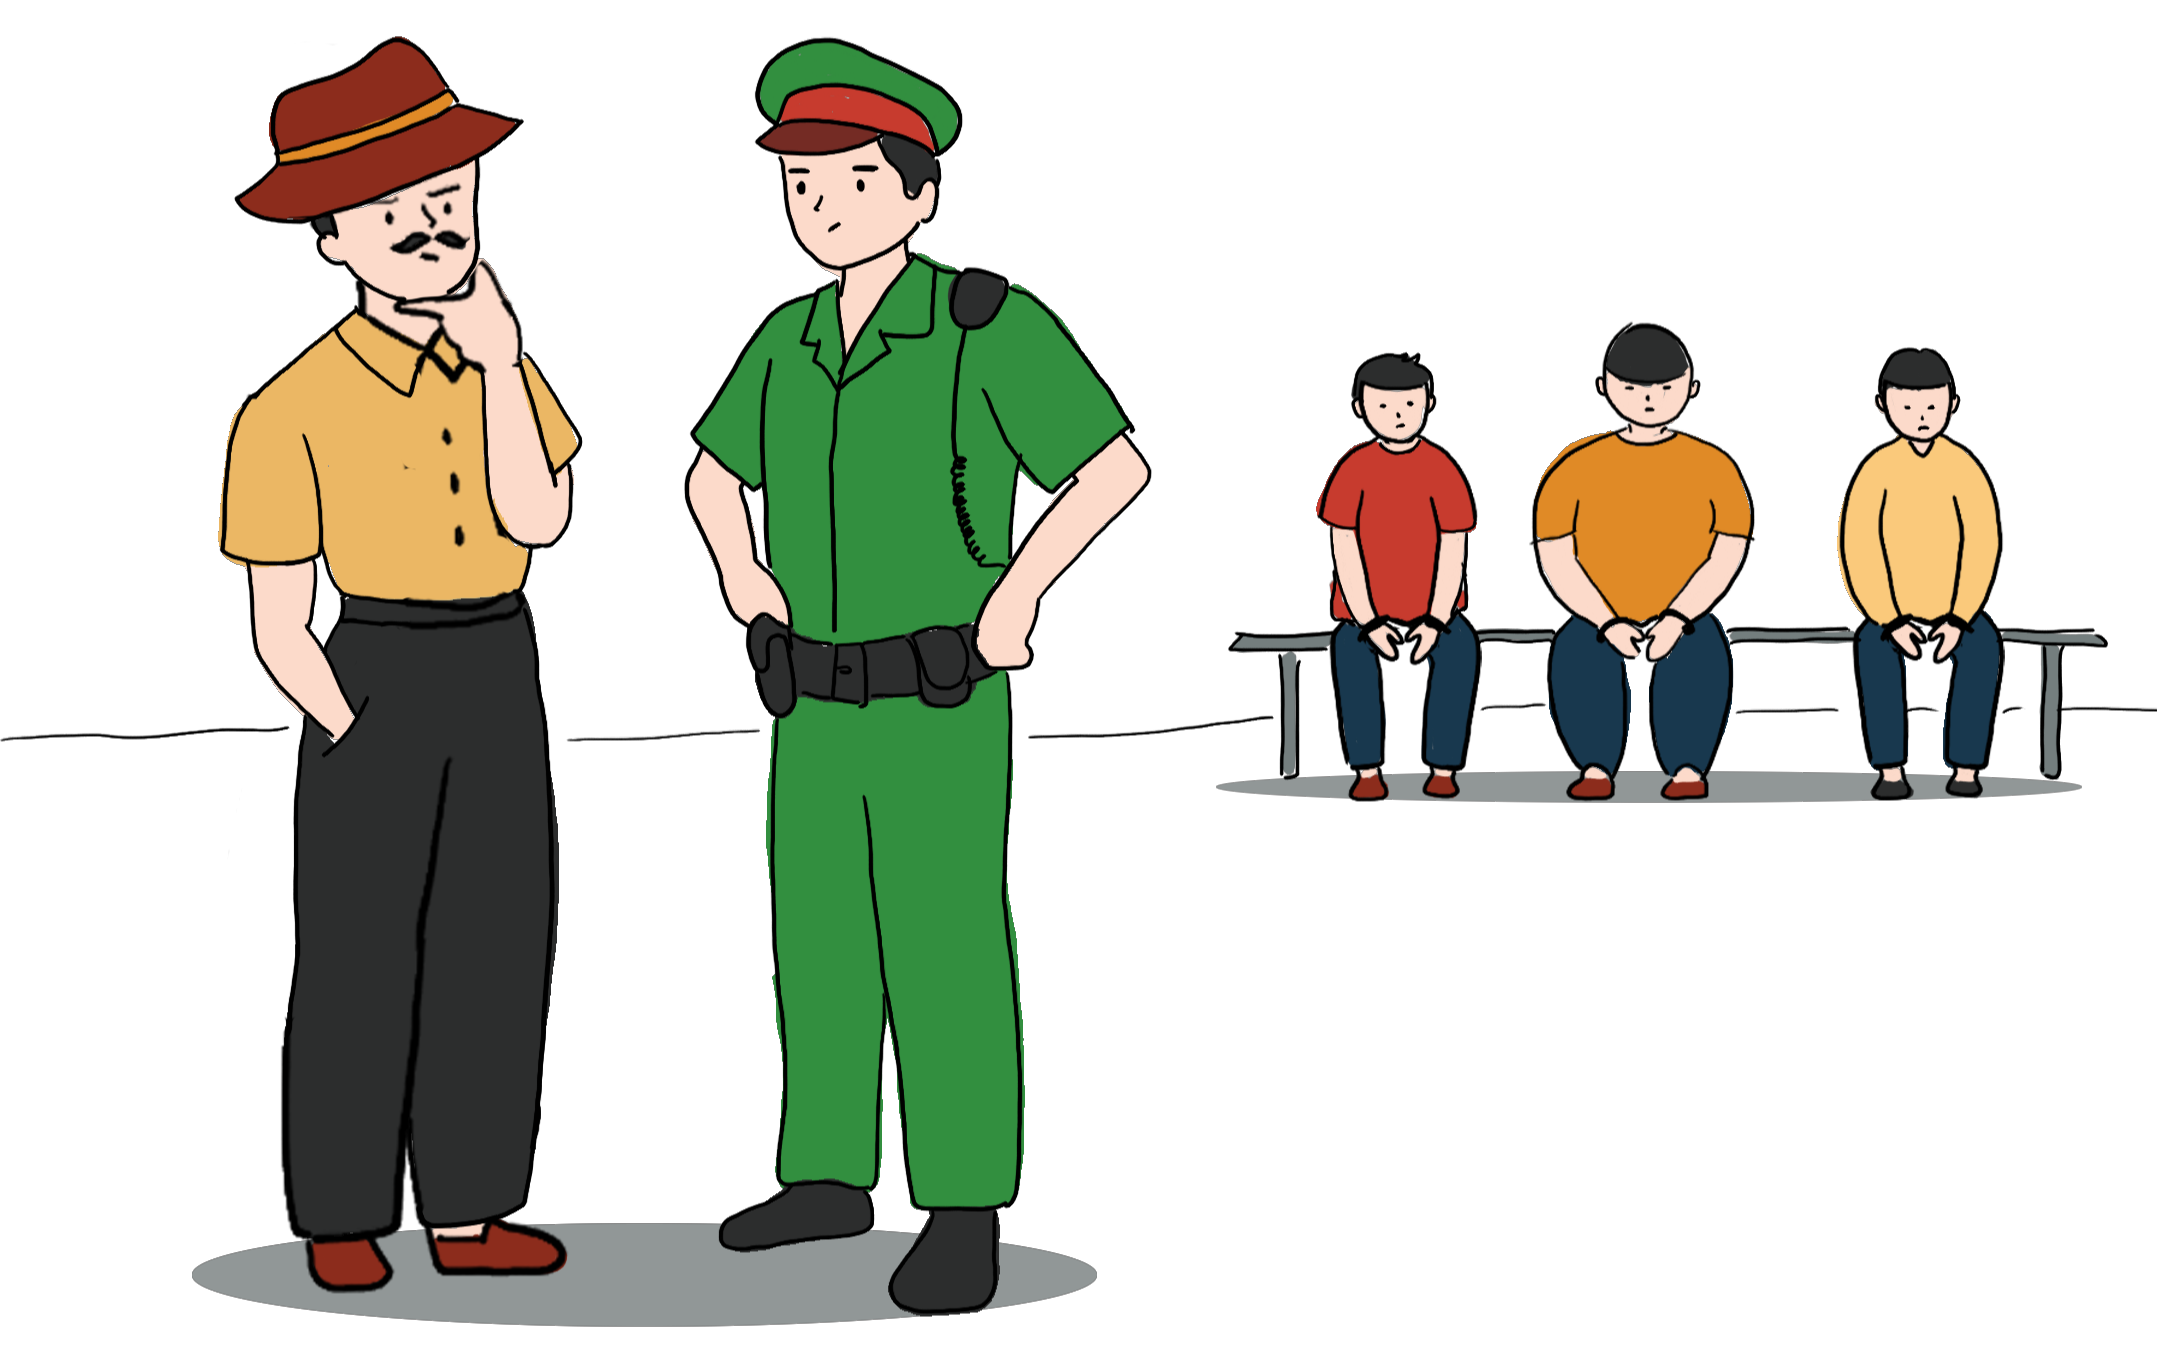
\includegraphics[width=1\linewidth]{xp}
		\vspace*{-10pt}
	\end{figure}
\end{multicols}
\newpage
%\vspace*{-10pt}
%{\color{toancuabi}\rule{1\linewidth}{0.1pt}}
\begingroup
\AddToShipoutPicture*{\put(115,672){
\includegraphics[scale=1]{../tieude11.pdf}}} 
\centering
\endgroup
\vspace*{35pt}

\begin{multicols}{2}
	$\pmb{1.}$ Các bạn nam mang kẹo tới lớp để tặng cho các bạn nữ. Bạn Phúc nói rằng mình đã mang tới đúng một nửa tổng số kẹo. Bạn Kiên nói rằng mình đã mang tới đúng một phần ba tổng số kẹo và chỉ chia kẹo của mình cho Mai và Tuyết, hơn nữa Mai được nhiều hơn so với Tuyết là $3$ chiếc kẹo. Em hãy chứng tỏ rằng có một bạn trong số Phúc và Kiên đã nhầm lẫn.
	\begin{figure}[H]
		\centering
		\vspace*{-5pt}
		\captionsetup{labelformat= empty, justification=centering}
		
\includegraphics[width=0.72\linewidth]{Pi7_bai1}
		\vspace*{-10pt}
	\end{figure}
	$\pmb{2.}$ Ba người thợ cùng đào một chiếc hố. Họ luân phiên lần lượt làm việc, mỗi người làm việc trong một thời gian nhất định. Nếu trong khi một người làm việc hai người còn lại cũng đồng thời đào hố thì hai người này sẽ đào được đúng một nửa hố. Hỏi nếu cả ba người cùng đồng thời đào thì họ sẽ làm nhanh hơn được bao nhiêu lần so với cách làm luân phiên ban đầu?
	\begin{figure}[H]
		\centering
		\vspace*{-5pt}
		\captionsetup{labelformat= empty, justification=centering}
		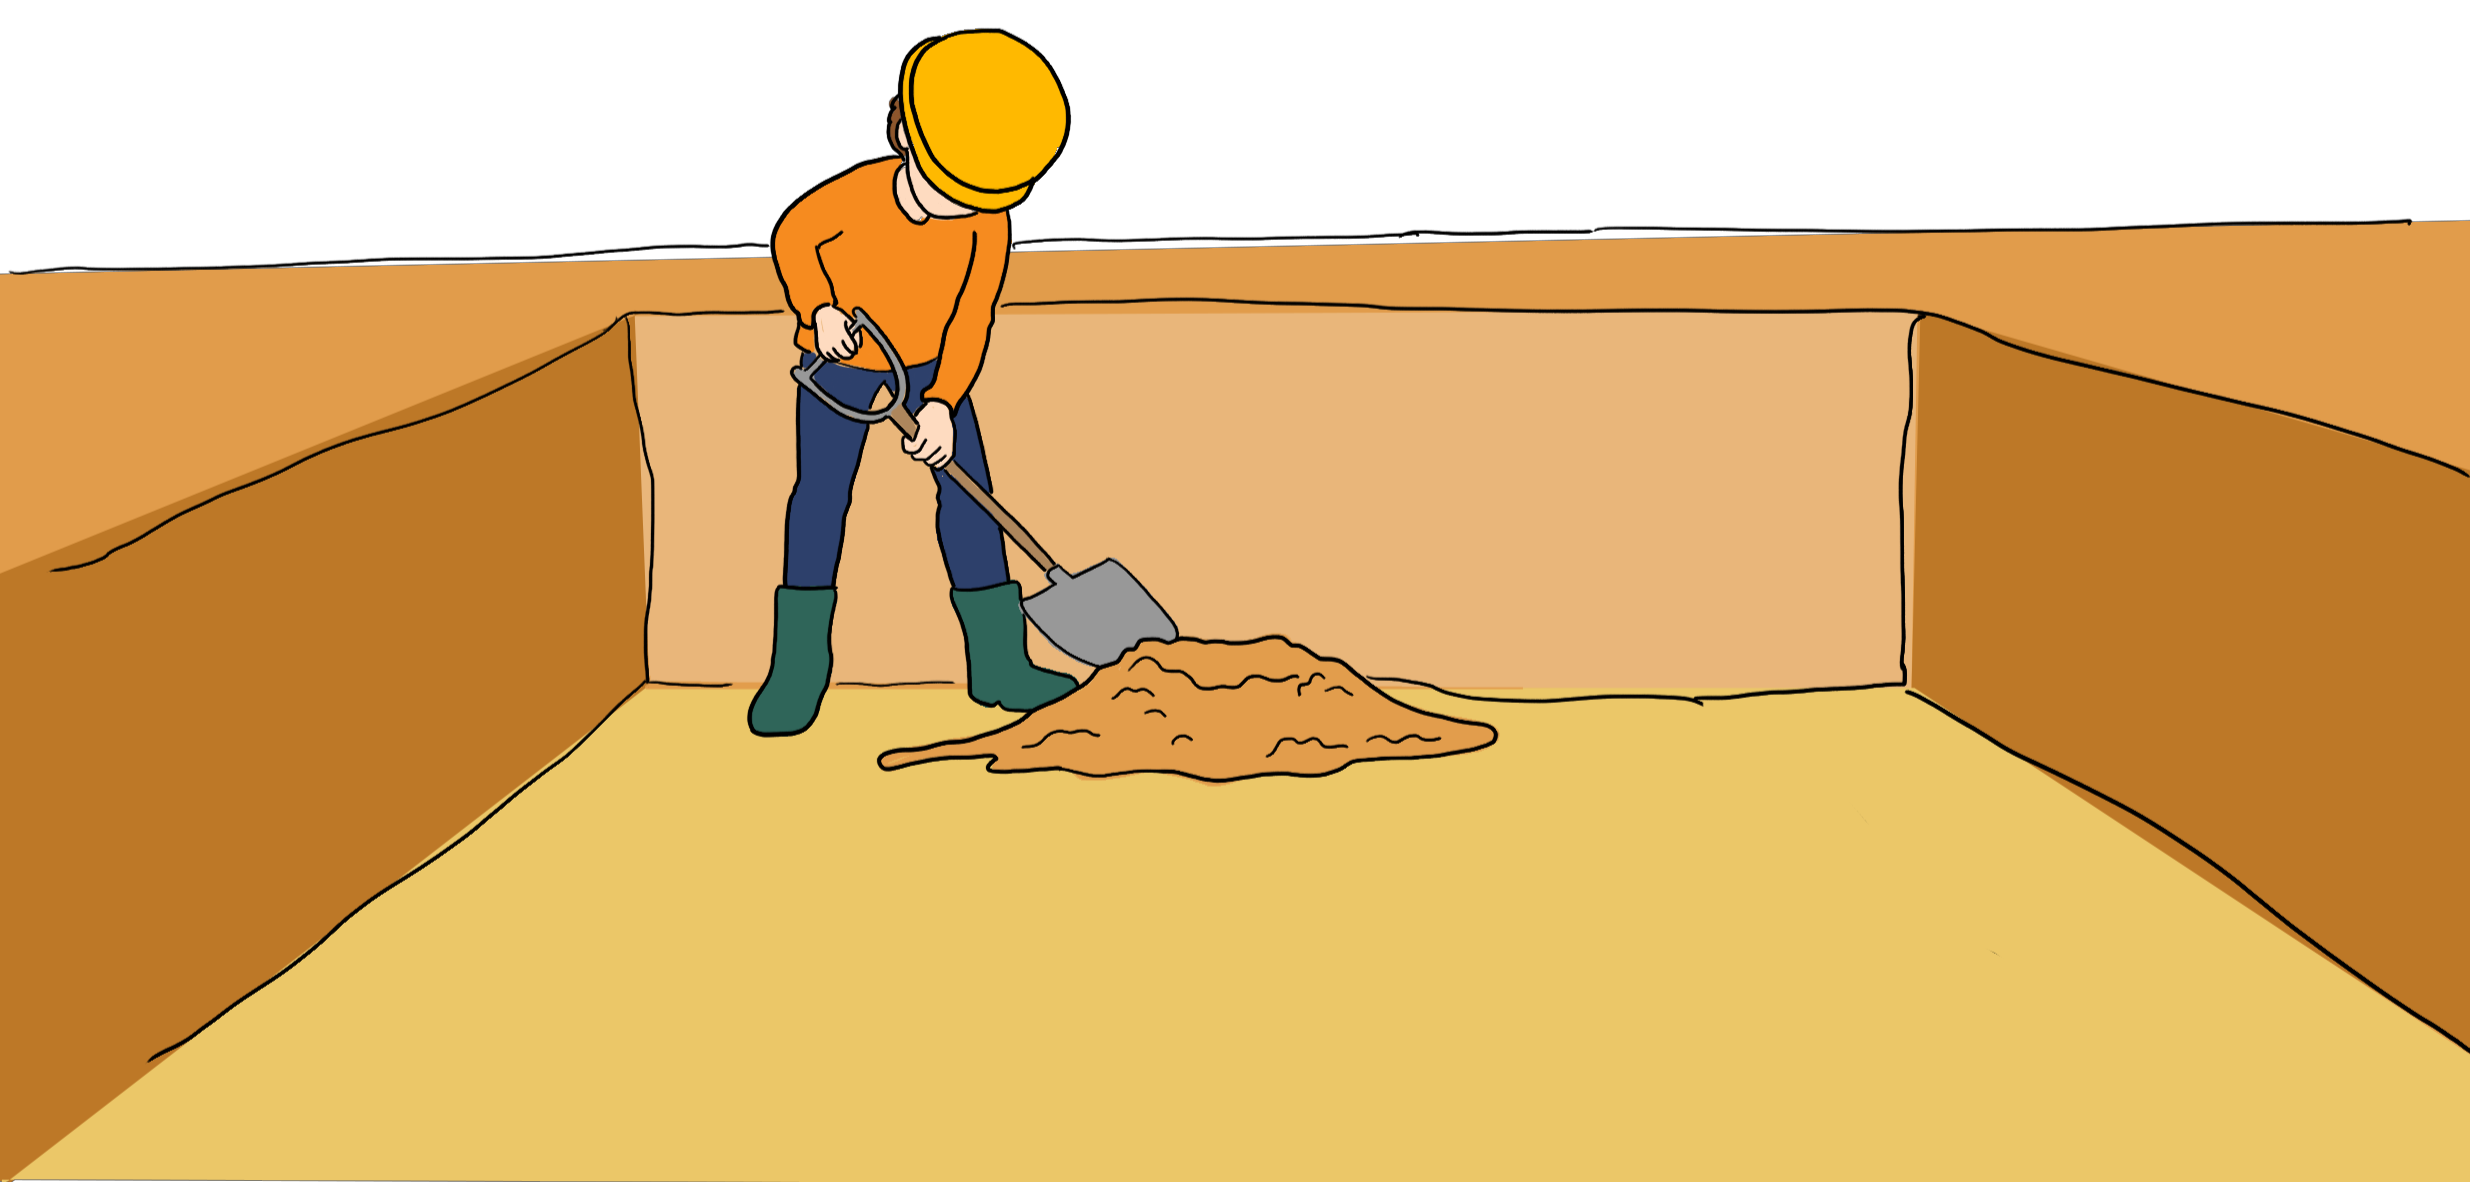
\includegraphics[width=1\linewidth]{Pi7_bai2}
		\vspace*{-15pt}
	\end{figure}
	$\pmb{3.}$ Ba bạn Gấu, Thỏ và Mèo cùng quyết định xây một con đường từ nhà tới bờ suối với chiều dài $160m$. Các bạn thoả thuận sẽ đầu tư cho dự án mở đường quan trọng này với công sức đều như nhau. Cuối cùng khi dự án hoàn thành, hoá ra bạn Thỏ đã xây được $60$ mét đường, bạn Mèo xây được $100$ mét đường, còn bạn Gấu mải ngủ đông nên không xây được mét nào. Tuy nhiên, Gấu mang tới đóng góp bằng tiền cho dự án là $16$ triệu đồng từ số mật ong bán được của mình. Hỏi hai bạn Mèo và bạn Thỏ cần phải phân chia số tiền cho nhau như thế nào?
	\begin{figure}[H]
		\centering
		\vspace*{-5pt}
		\captionsetup{labelformat= empty, justification=centering}
		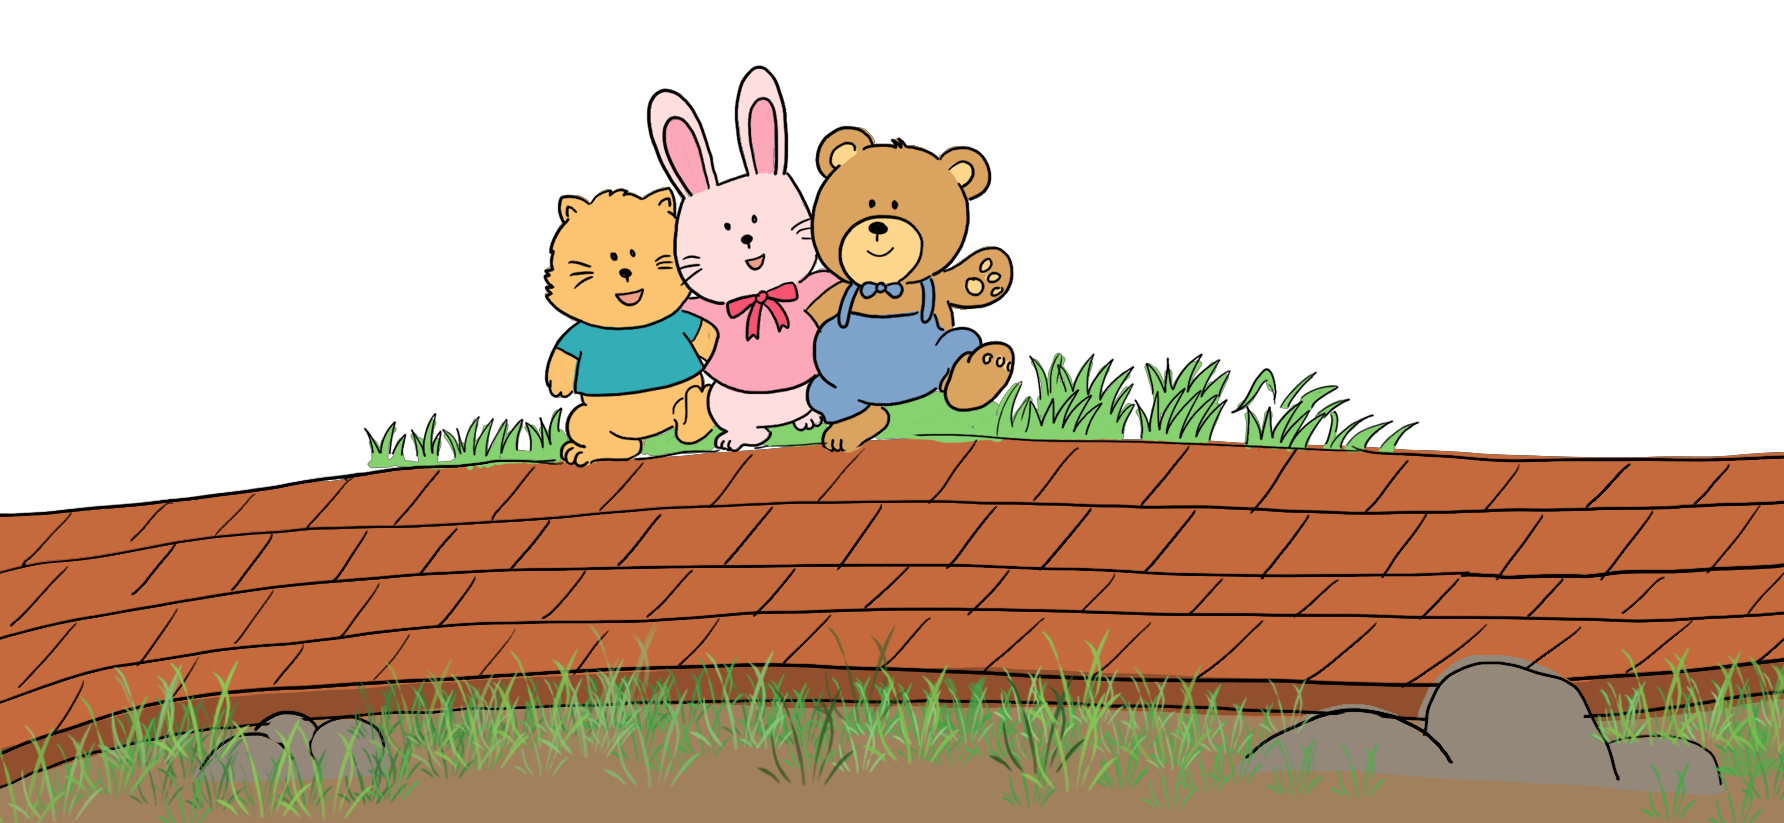
\includegraphics[width=1\linewidth]{Pi7_bai3}
		\vspace*{-15pt}
	\end{figure}
	$\pmb{4.}$ Bé Ly phải đi trồng hoa vào một hàng các chậu rất dài đặt thành hàng dọc ở công viên. Bé được giao nhiệm vụ là phải trồng hai loại hoa khác nhau vào hai chiếc chậu nếu giữa hai chậu này có đúng hai chiếc chậu, hoặc đúng ba chiếc chậu, hoặc đúng năm chiếc chậu khác. Hỏi bé Ly phải cần ít nhất bao nhiêu loại hoa để thực hiện được nhiệm vụ?
	\begin{figure}[H]
		\centering
		\vspace*{-5pt}
		\captionsetup{labelformat= empty, justification=centering}
		
\includegraphics[width=0.5\linewidth]{Pi7_bai4}
		\vspace*{-10pt}
	\end{figure}
	$\pmb{5.}$ Trước một trận bóng đá giữa hai đội Xóm Đông và Xóm Bắc có $5$ dự đoán kết quả được đưa ra:
	\vskip 0.1cm
	$a)$	Sẽ không có tỷ số hoà;
	\vskip 0.1cm
	$b)$	Đội Xóm Đông sẽ bị thủng lưới;
	\vskip 0.1cm
	$c)$	Đội Xóm Bắc sẽ thắng;
	\vskip 0.1cm
	$d)$	Đội Xóm Bắc sẽ không thua;
	\vskip 0.1cm
	$e)$	Trong trận bóng sẽ có đúng $3$ bàn thắng được ghi.
	\vskip 0.1cm
	Sau khi trận bóng kết thúc, hoá ra chỉ có đúng $3$ dự đoán là chính xác. Vậy trận đấu đã kết thúc với tỷ số như thế nào?
	\begin{figure}[H]
		\centering
		\vspace*{-5pt}
		\captionsetup{labelformat= empty, justification=centering}
		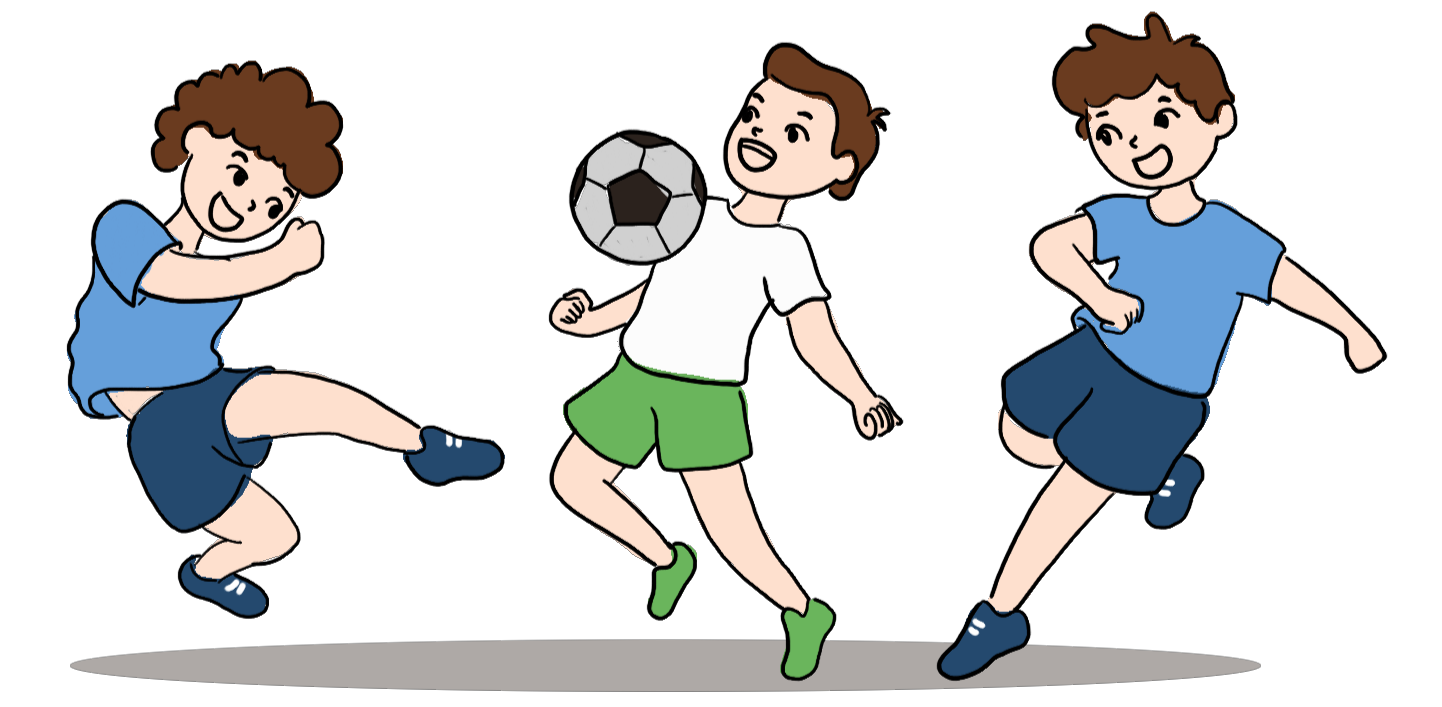
\includegraphics[width=1\linewidth]{Pi7_bai5}
		\vspace*{-15pt}
	\end{figure}
	$\pmb{6.}$ 	Tại trại hè có $20$ em học sinh tham gia trò chơi Điệp viên tí hon diễn ra trong $2$ tuần. Mỗi Điệp viên tí hon sẽ theo dõi và viết báo cáo tỉ mỉ về sở thích cá nhân của $10$ em khác trong số $20$ em này để nộp cho Sở chỉ huy. Em hãy chứng tỏ rằng có ít nhất $10$ cặp Điệp viên tí hon đã theo dõi lẫn nhau và viết báo cáo về nhau.
	\begin{figure}[H]
		\centering
		\vspace*{-5pt}
		\captionsetup{labelformat= empty, justification=centering}
		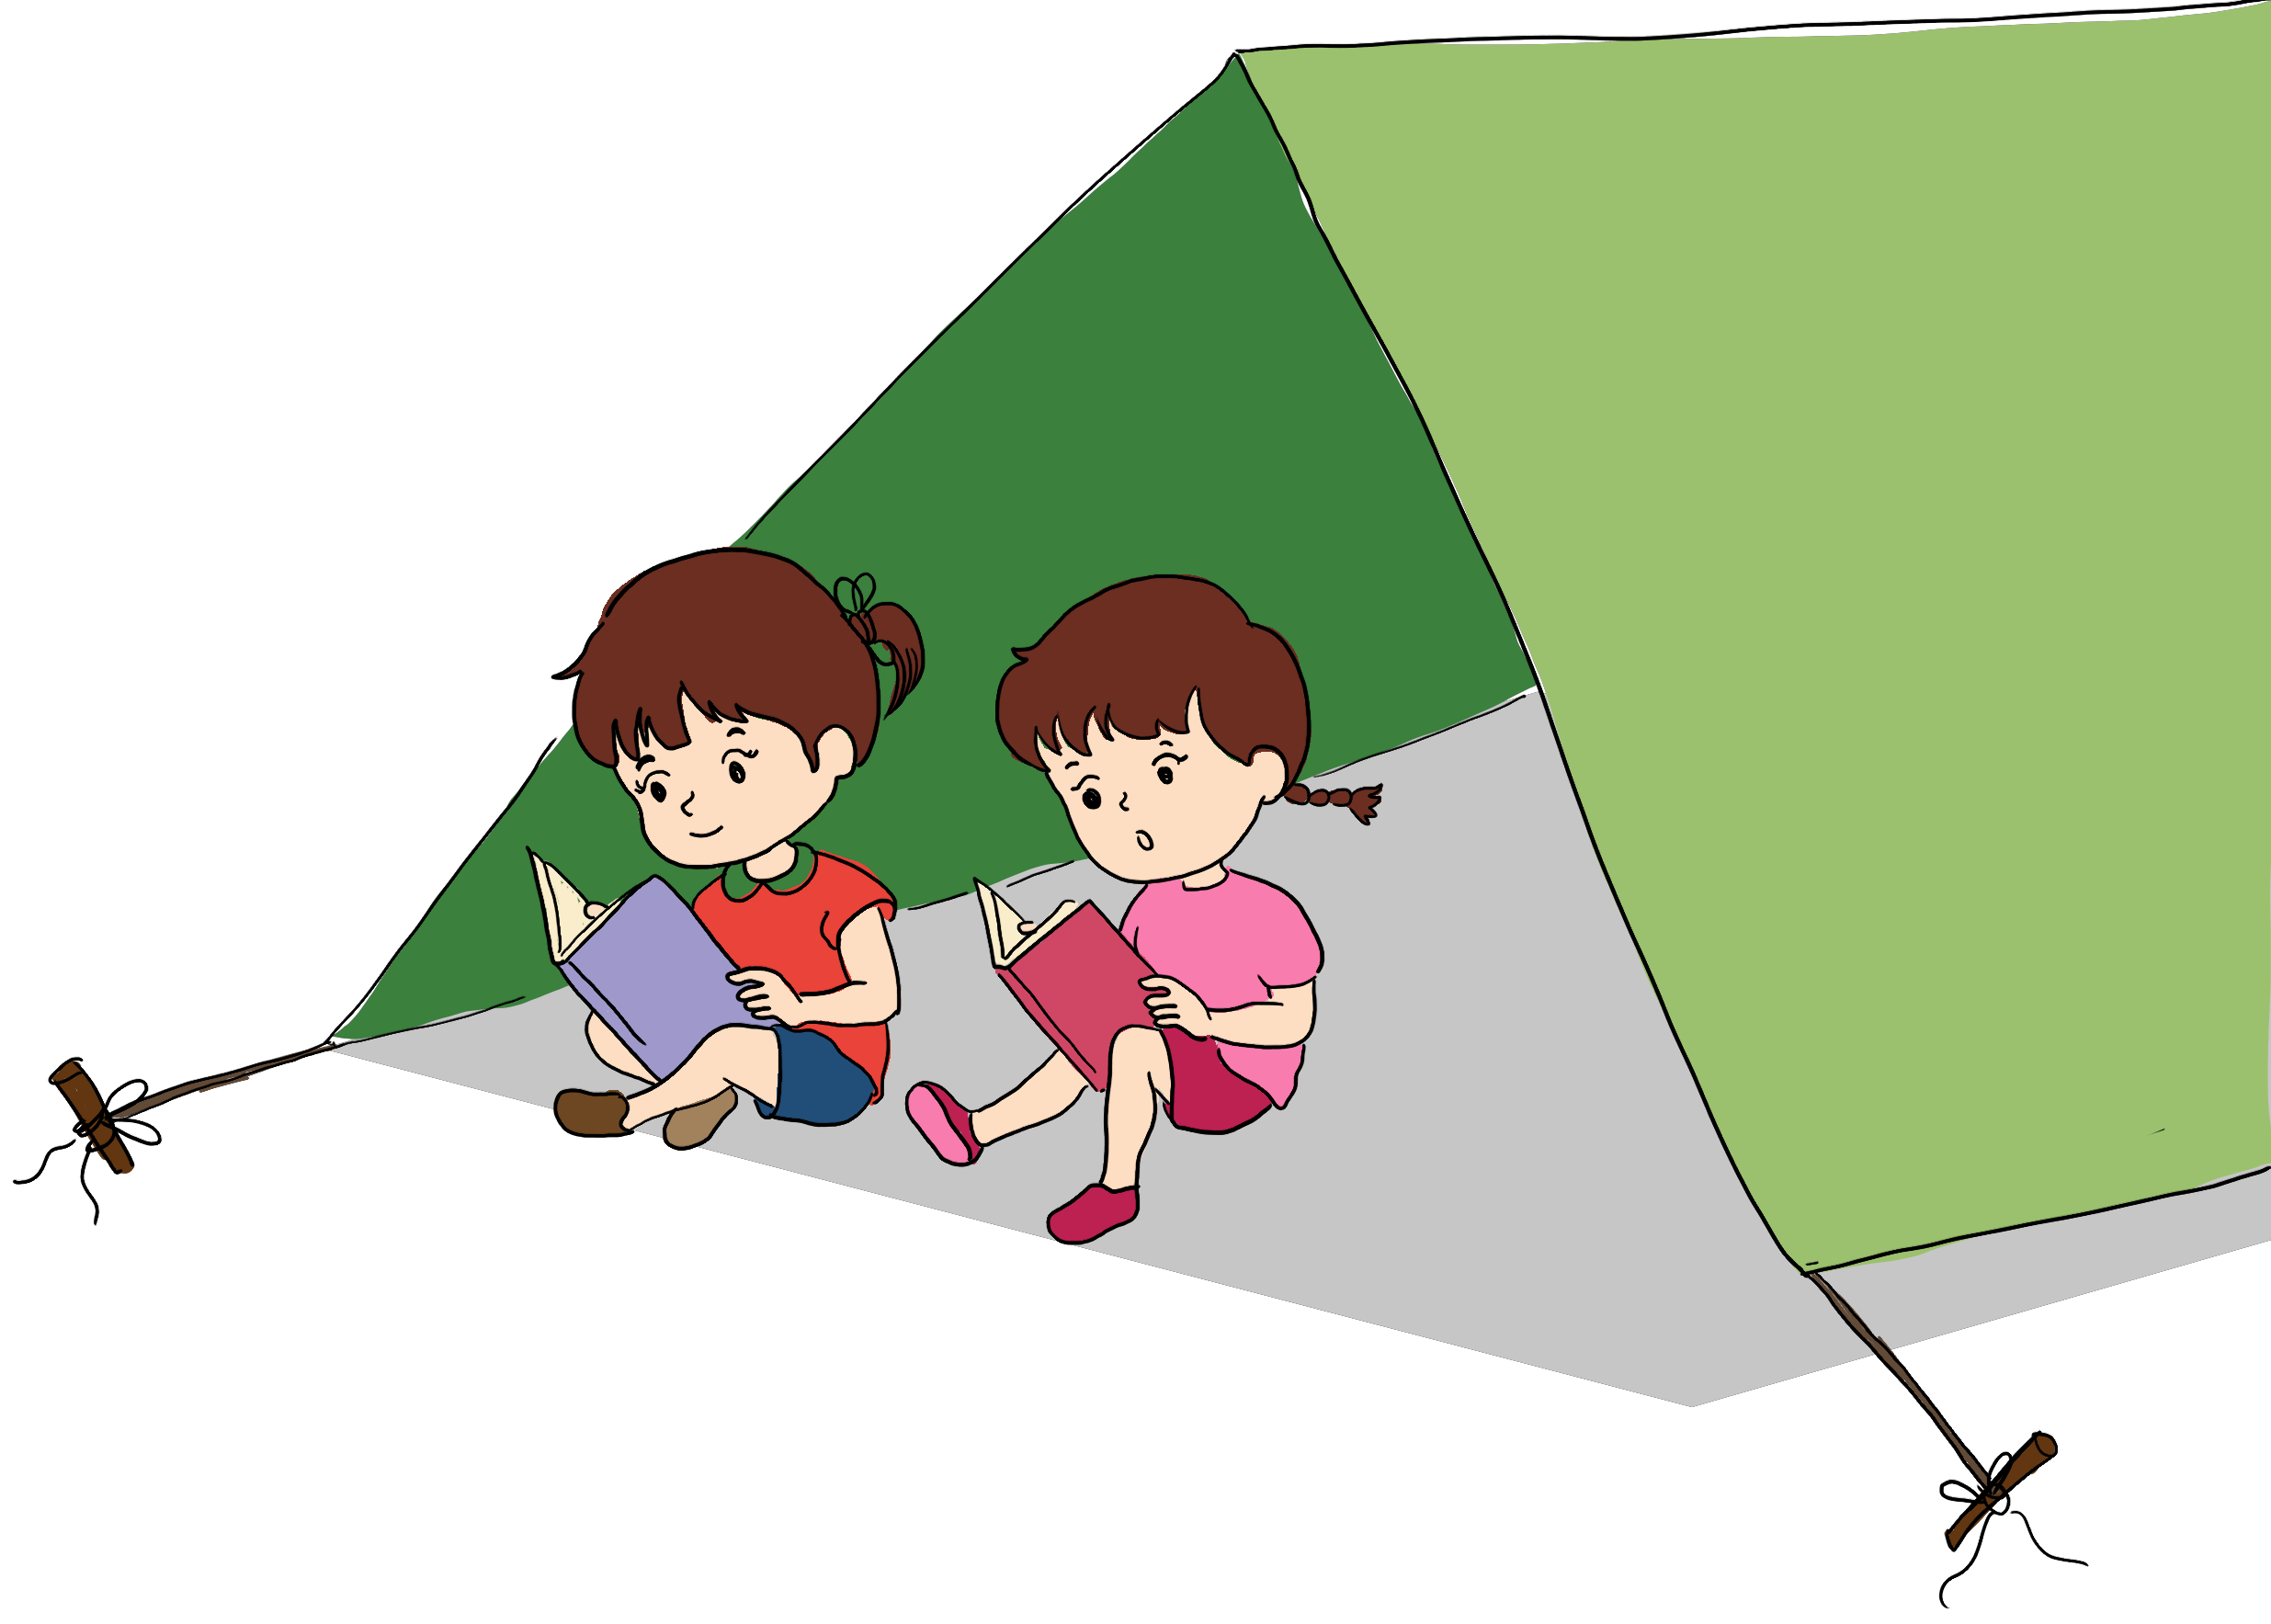
\includegraphics[width=1\linewidth]{Pi7_bai6}
		\vspace*{-5pt}
	\end{figure}
\end{multicols}
\vspace*{-10pt}
{\color{toancuabi}\rule{1\linewidth}{0.1pt}}
%\newpage
\begingroup
\AddToShipoutPicture*{\put(112,370){
\includegraphics[scale=1]{../tieude2.pdf}}} 
\centering
\endgroup
\vspace*{75pt}

\begin{multicols}{2}
	$\pmb{1.}$	Pinocchio và Pierrot thi chạy với nhau. Pierrot chạy suốt cả quãng đường với cùng một tốc độ, còn Pinocchio chạy nhanh gấp đôi Pierrot trong nửa đầu quãng đường, và nửa sau lại chậm bằng nửa Pierrot. Hỏi ai đã thắng?
	\begin{figure}[H]
		\centering
		\vspace*{-5pt}
		\captionsetup{labelformat= empty, justification=centering}
		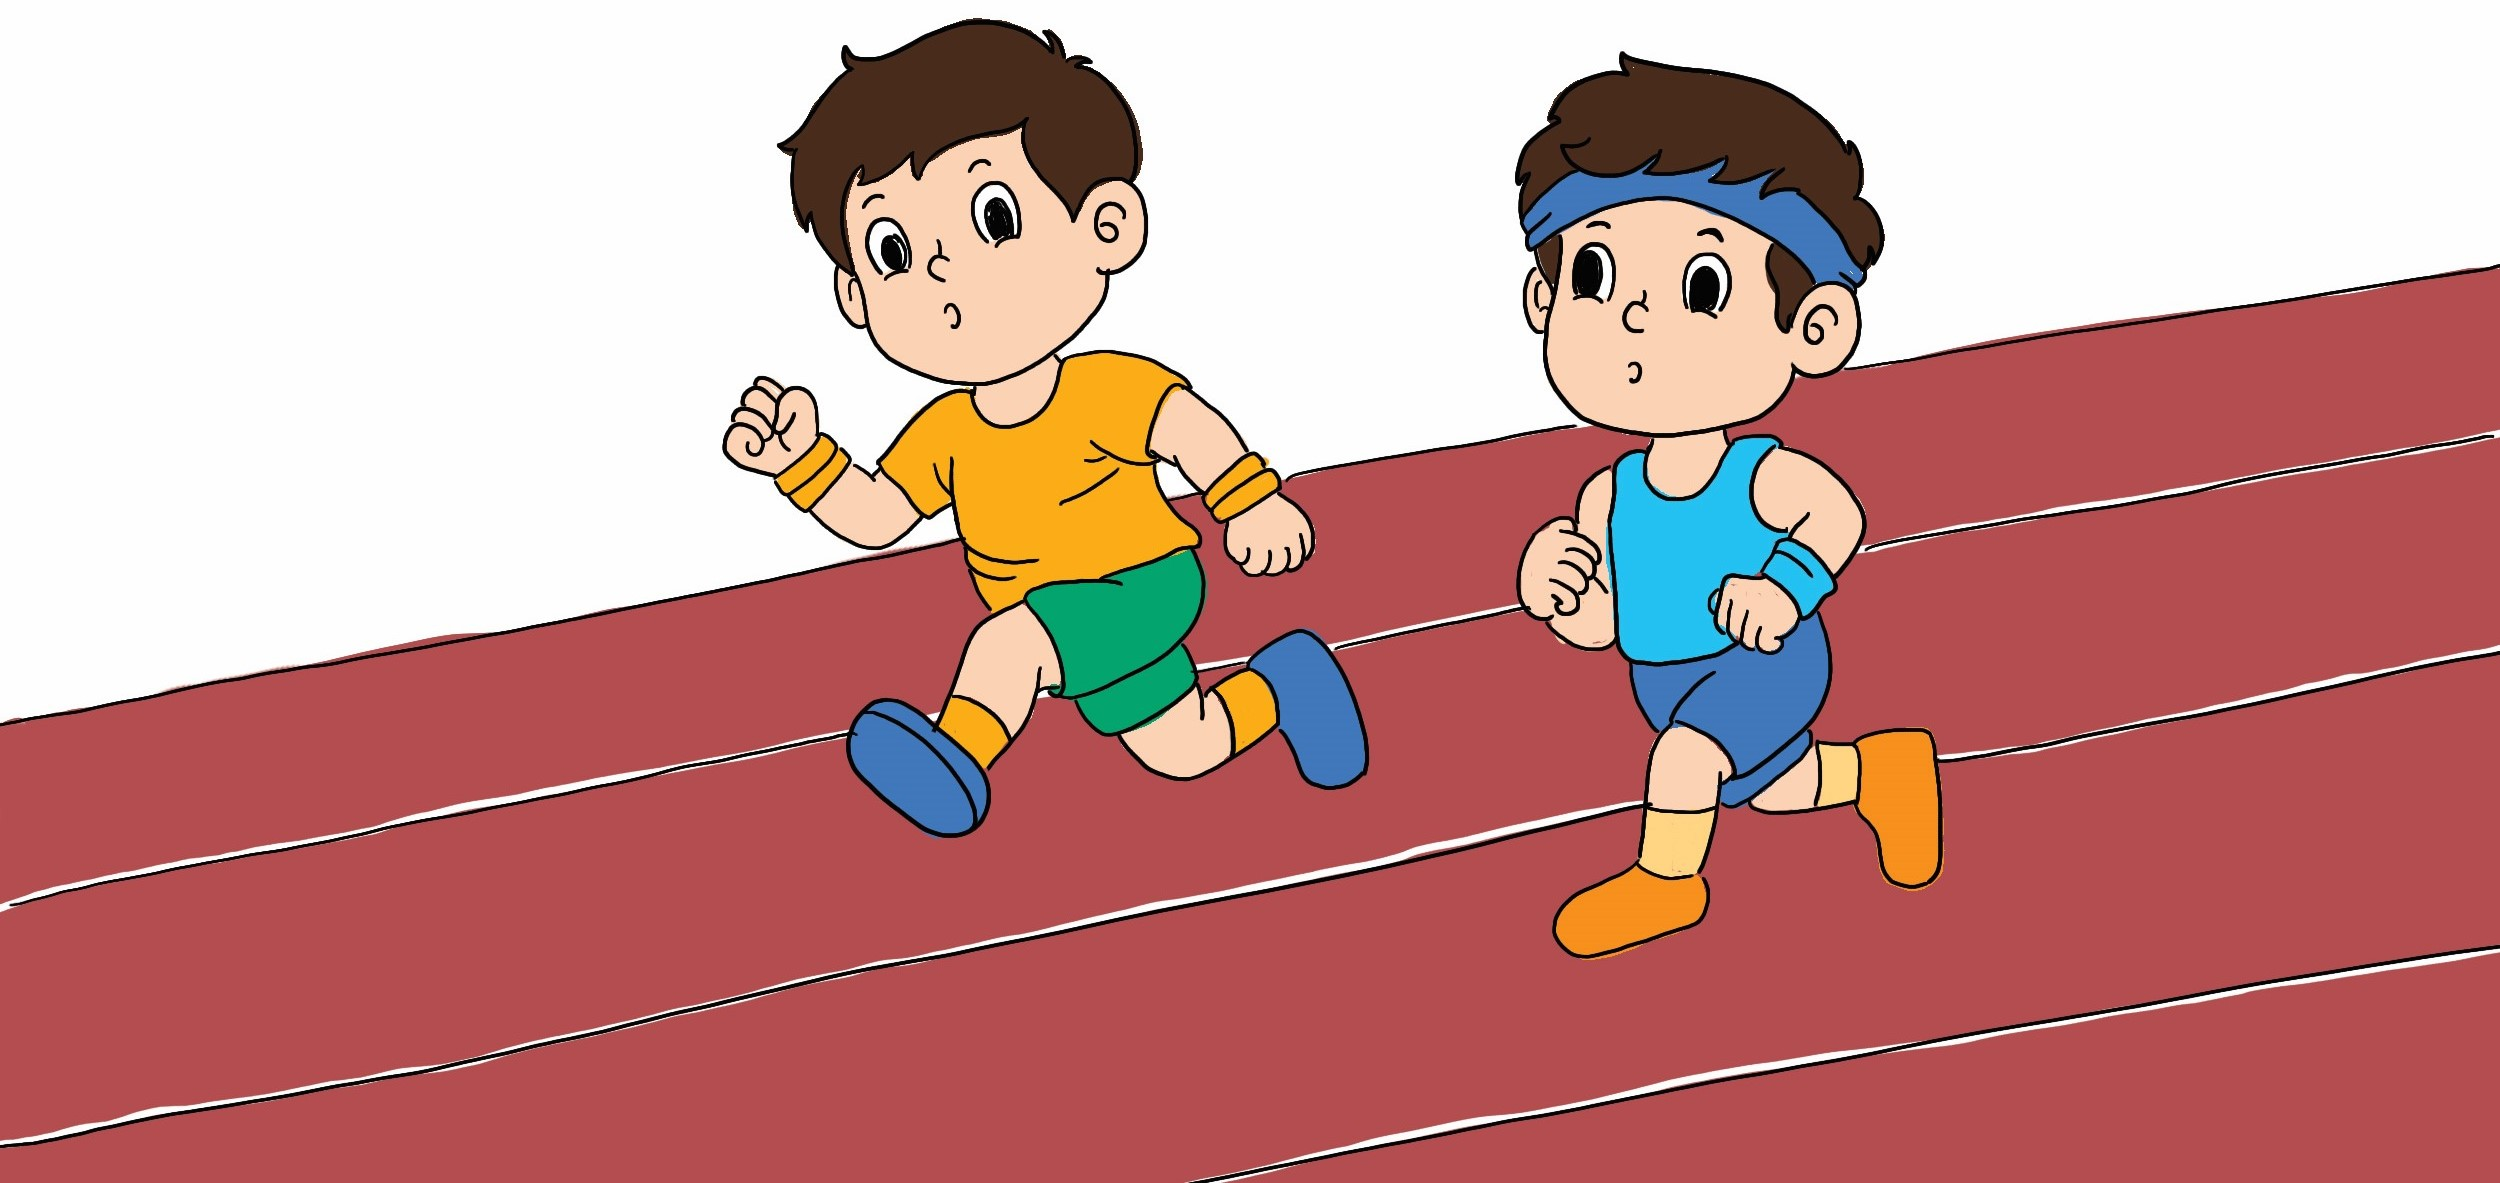
\includegraphics[width=1\linewidth]{Pi4_bai1}
		\vspace*{-15pt}
	\end{figure}
	\textit{Lời giải.} Trong nửa sau của cuộc đua, Pinocchio đã mất một khoảng thời gian đúng bằng thời gian Pierrot dành cho toàn bộ cuộc đua. Nhưng Pinocchio cũng đã mất một khoảng thời gian trong nửa đầu của cuộc đua. Vì vậy, Pierrot đã thắng. 
	\vskip 0.1cm
	$\pmb{2.}$ ``Còn quá sớm để các em nhìn thấy điều thần kỳ sau đây của thế giới pháp sư," cô giáo McGonagall  nói với $33$ học trò của mình ở ngôi trường Hogwarts đào tạo Phù thủy, và vung cây đũa thần ra lệnh: ``Nào, các em hãy nhắm mắt lại!" Tất cả học trò nam và một phần ba học trò nữ đều nhắm mắt phải. Tất cả học trò nữ và một phần ba các học trò nam đều nhắm mắt trái. Hỏi có bao nhiêu học trò đã nhìn thấy những gì còn quá sớm để nhìn thấy?
	\begin{figure}[H]
		\centering
		\vspace*{-10pt}
		\captionsetup{labelformat= empty, justification=centering}
		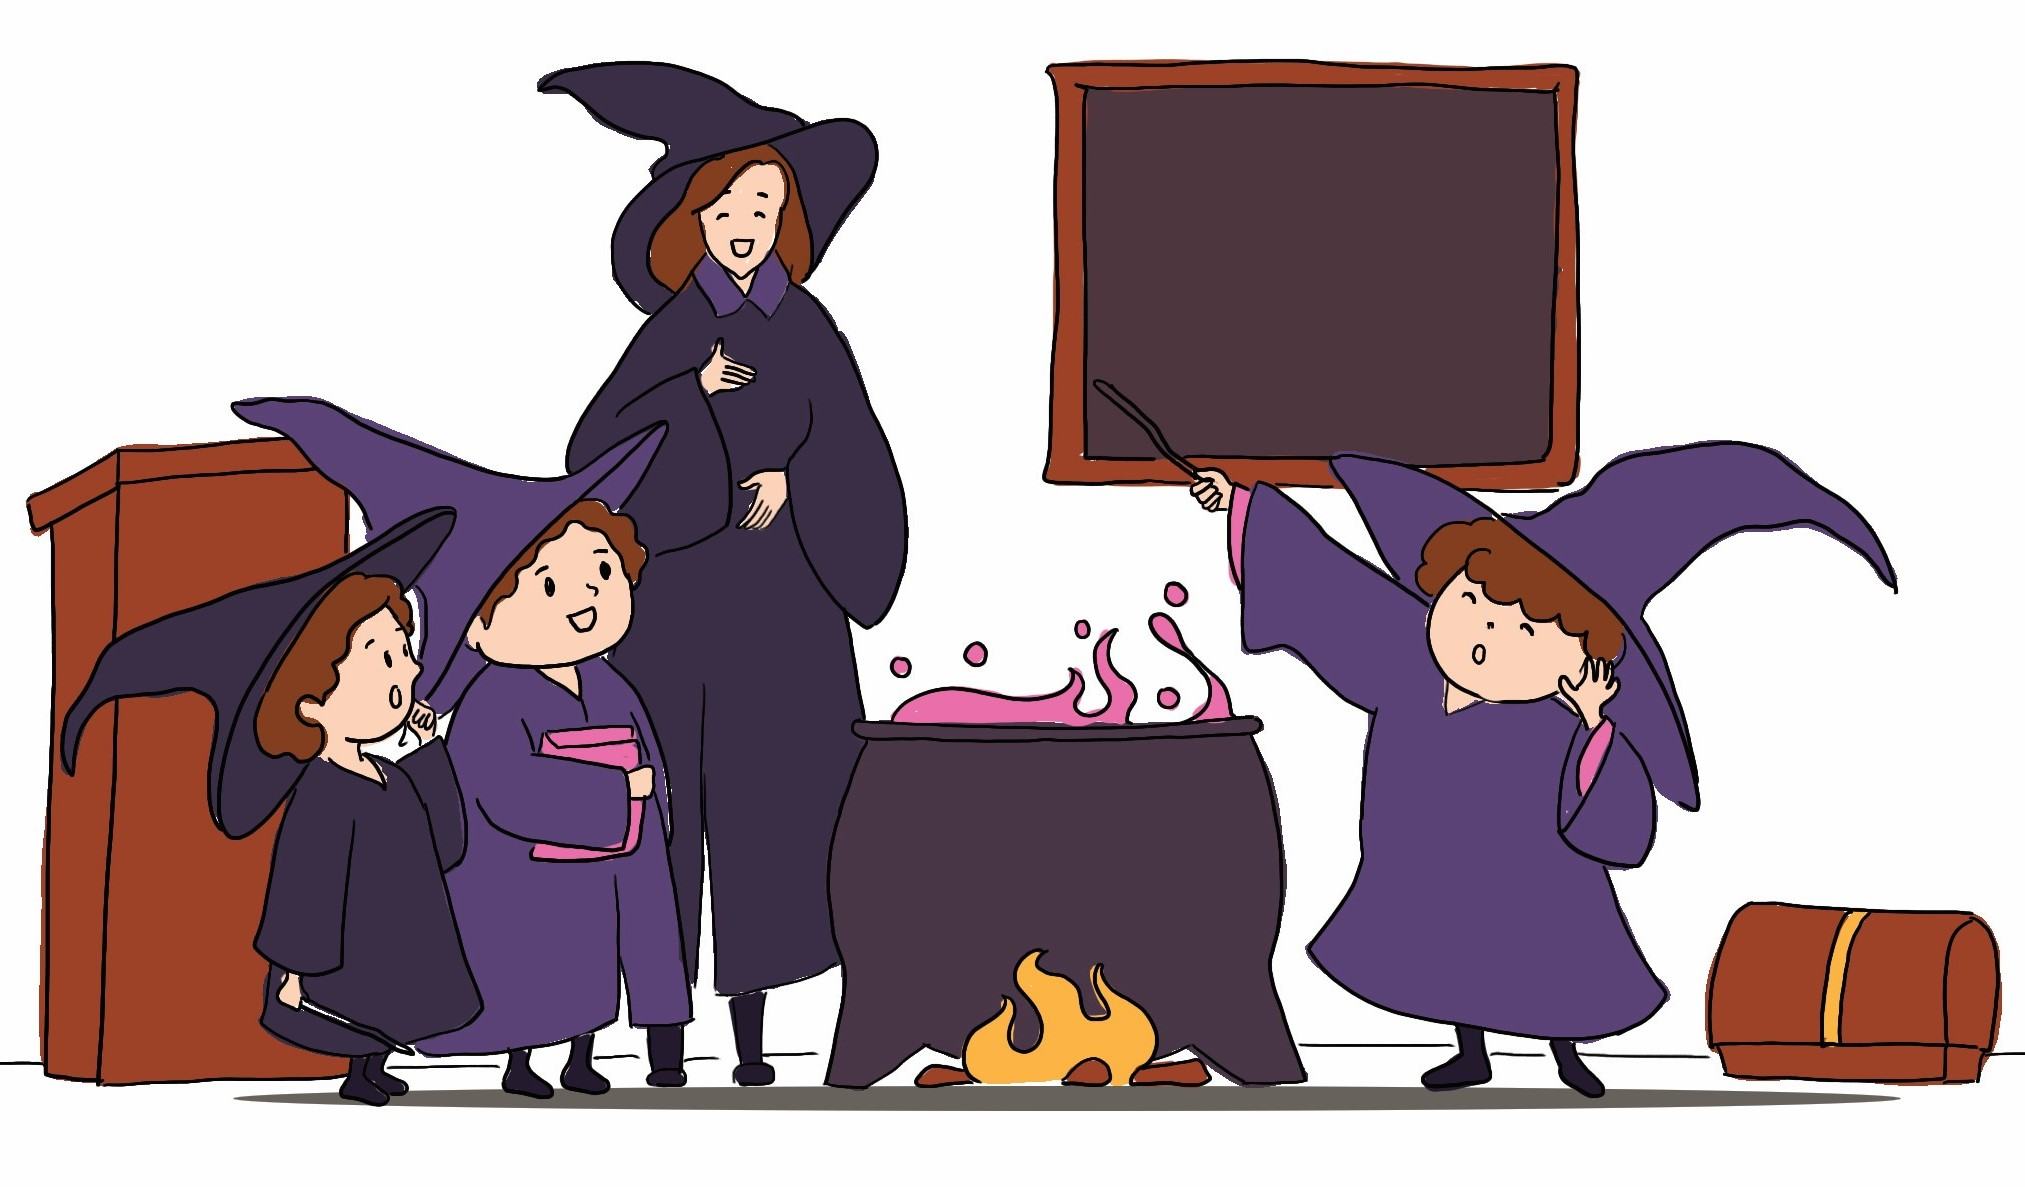
\includegraphics[width=1\linewidth]{Pi4_bai2}
		\vspace*{-15pt}
	\end{figure}
	\textit{Lời giải.} Có $2/3$ nữ sinh đã nhìn bằng mắt phải và $2/3$ nam sinh đã nhìn bằng mắt trái thấy điều còn quá sớm để nhìn thấy. Do đó, tổng cộng, $2/3$ tổng số học sinh đã không nhắm  một mắt -- vậy có $22$ học sinh đã nhìn thấy điều này.
	\vskip 0.1cm
	$\pmb{3.}$ 	Bác Tư múc ra ba thìa sữa từ một ly sữa đầy và đổ chúng vào một ly đựng cà phê nguyên chất và khuấy đều. Sau đó bác múc ba thìa hỗn hợp thu được và đổ lại vào ly sữa. Hỏi bây giờ thứ gì nhiều hơn: cà phê trong ly đựng sữa hay sữa trong ly đựng cà phê?
	\begin{figure}[H]
		\centering
		\vspace*{5pt}
		\captionsetup{labelformat= empty, justification=centering}
		
\includegraphics[width=1\linewidth]{Pi4_bai3}
		\vspace*{-15pt}
	\end{figure}
	\textit{Lời giải.} Sau lần đổ thứ hai, lượng chất lỏng trong từng ly không thay đổi so với ban đầu nên lượng cà phê  có  trong ly sữa chính xác bằng lượng sữa đã được lấy ra từ đó. Vì vậy, cuối cùng, lượng cà phê trong sữa cũng nhiều như lượng sữa trong cà phê.
	\vskip 0.1cm
	$\pmb{4.}$ Ma xó Brownie là một nhân vật trong văn hóa dân gian Anh và một số quốc gia khác. Đó là một dạng Phúc thần (ma thiện), tiểu yêu nghịch ngợm, thường mô tả là bé tí hon, có da nâu, ăn mặc tuềnh toàng, sinh sống gần gũi với con người, và là thần hộ mệnh cho các gia đình. Các Brownies có một xã hội thu nhỏ riêng và thường tổ chức những cuộc họp bí mật tại một tảng đá nào đó để con người không để ý tới. 
	\vskip 0.1cm
	Trong một tòa nhà bảy tầng nọ cũng có rất nhiều ma xó Brownies sinh sống. Thang máy chạy giữa tầng một và tầng cuối, dừng lại ở mỗi tầng. Ở mỗi tầng, bắt đầu từ tầng đầu tiên, có một chú Brownie bước vào thang máy, nhưng không có chú nào bước ra ngoài. Thang máy cứ di chuyển liên tục như vậy cho đến khi chú Brownie thứ một nghìn bước vào thang máy thì thang máy dừng lại. Hỏi điều này đã xảy ra ở tầng nào?
	\begin{figure}[H]
		\centering
		\vspace*{-5pt}
		\captionsetup{labelformat= empty, justification=centering}
		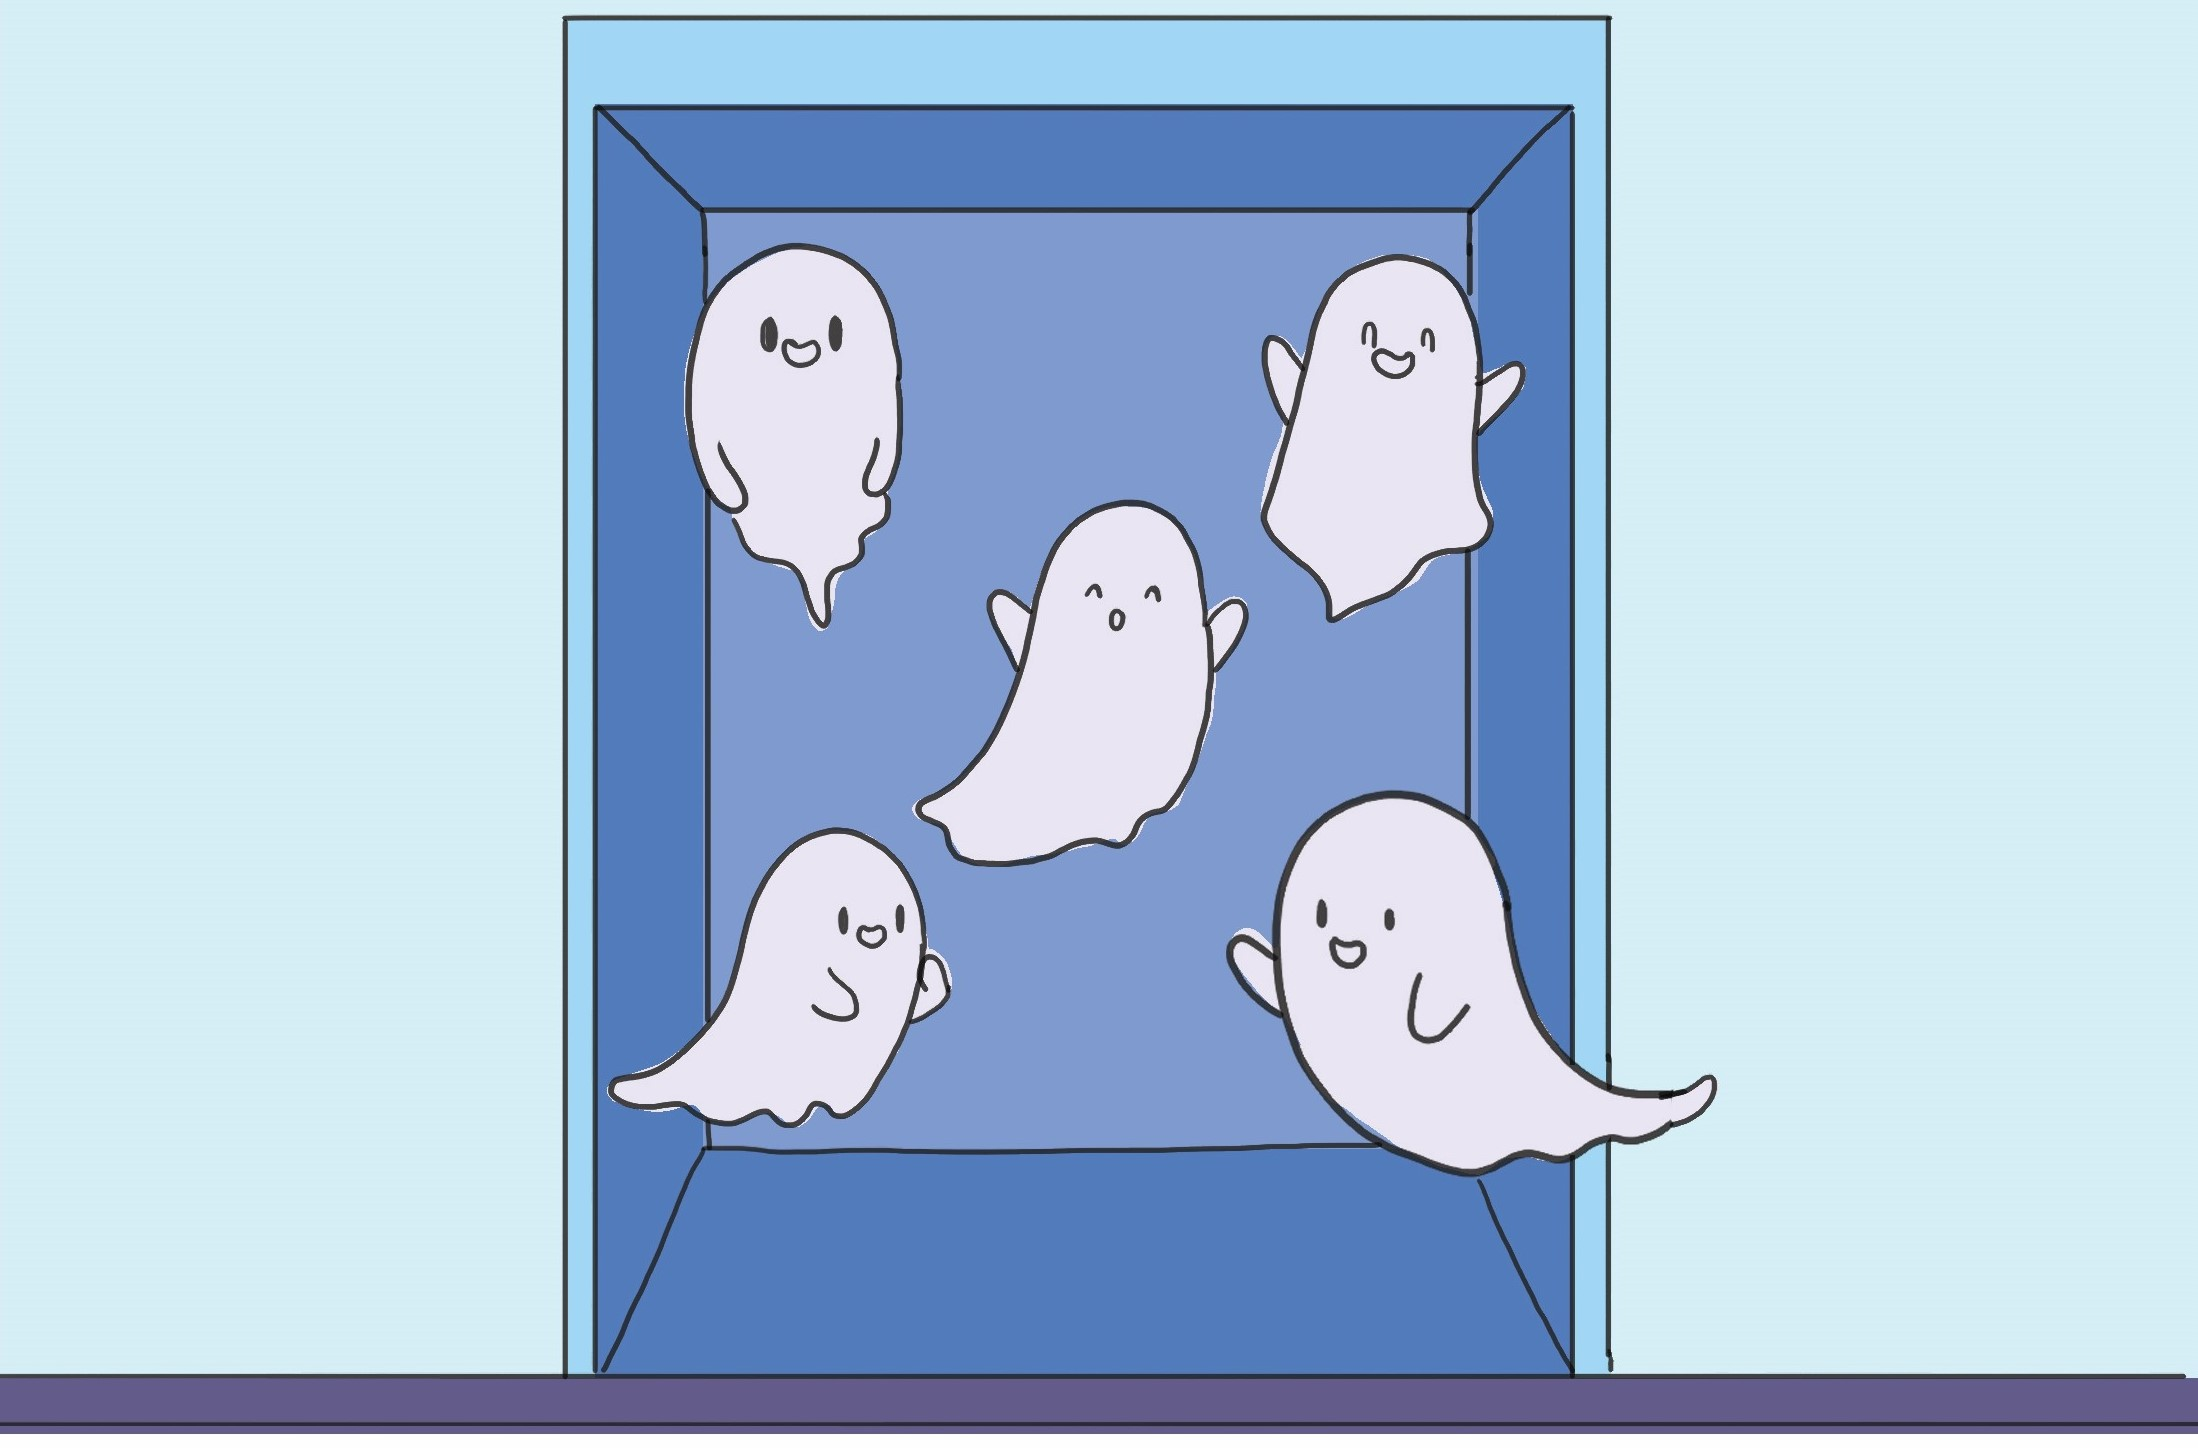
\includegraphics[width=1\linewidth]{Pi4_bai4}
		\vspace*{-20pt}
	\end{figure}
	\textit{Lời giải.} 	Các em hãy thử tìm xem có bao nhiêu chú Brownie trong thang máy trong một chuyến đi từ tầng một đến tầng bảy và ngược lại, cho đến thời điểm thang máy quay trở lại tầng một. Ở tầng một và tầng bảy, có một chú Brownies bước vào, và ở tất cả các tầng khác, mỗi tầng đều có  hai chú Brownie bước vào. Do đó, $12$ chú Brownies vào thang máy trong một chuyến đi lên và xuống như vậy. 
	\vskip 0.1cm
	Ta có $1000 = 83 \times 12 + 4$. Vì vậy, sau $83$ lần đi, $4$ chú Brownies nữa vẫn sẽ có thể vào thang máy: ở tầng một, tầng hai, tầng ba và tầng bốn. 
	Như vậy thang máy đã dừng ở tầng bốn.
	\vskip 0.1cm
	$\pmb{5.}$ Có $40$ con thú sống trong rừng gồm cáo, sói, thỏ rừng và lửng. Hàng năm, các con thú tổ chức vũ hội hóa trang: mỗi con đeo một chiếc mặt nạ của một loài động vật khác và trong hai năm liên tiếp không con nào đeo cùng một chiếc mặt nạ của cùng một loài.
	\begin{figure}[H]
		\centering
		\vspace*{-5pt}
		\captionsetup{labelformat= empty, justification=centering}
		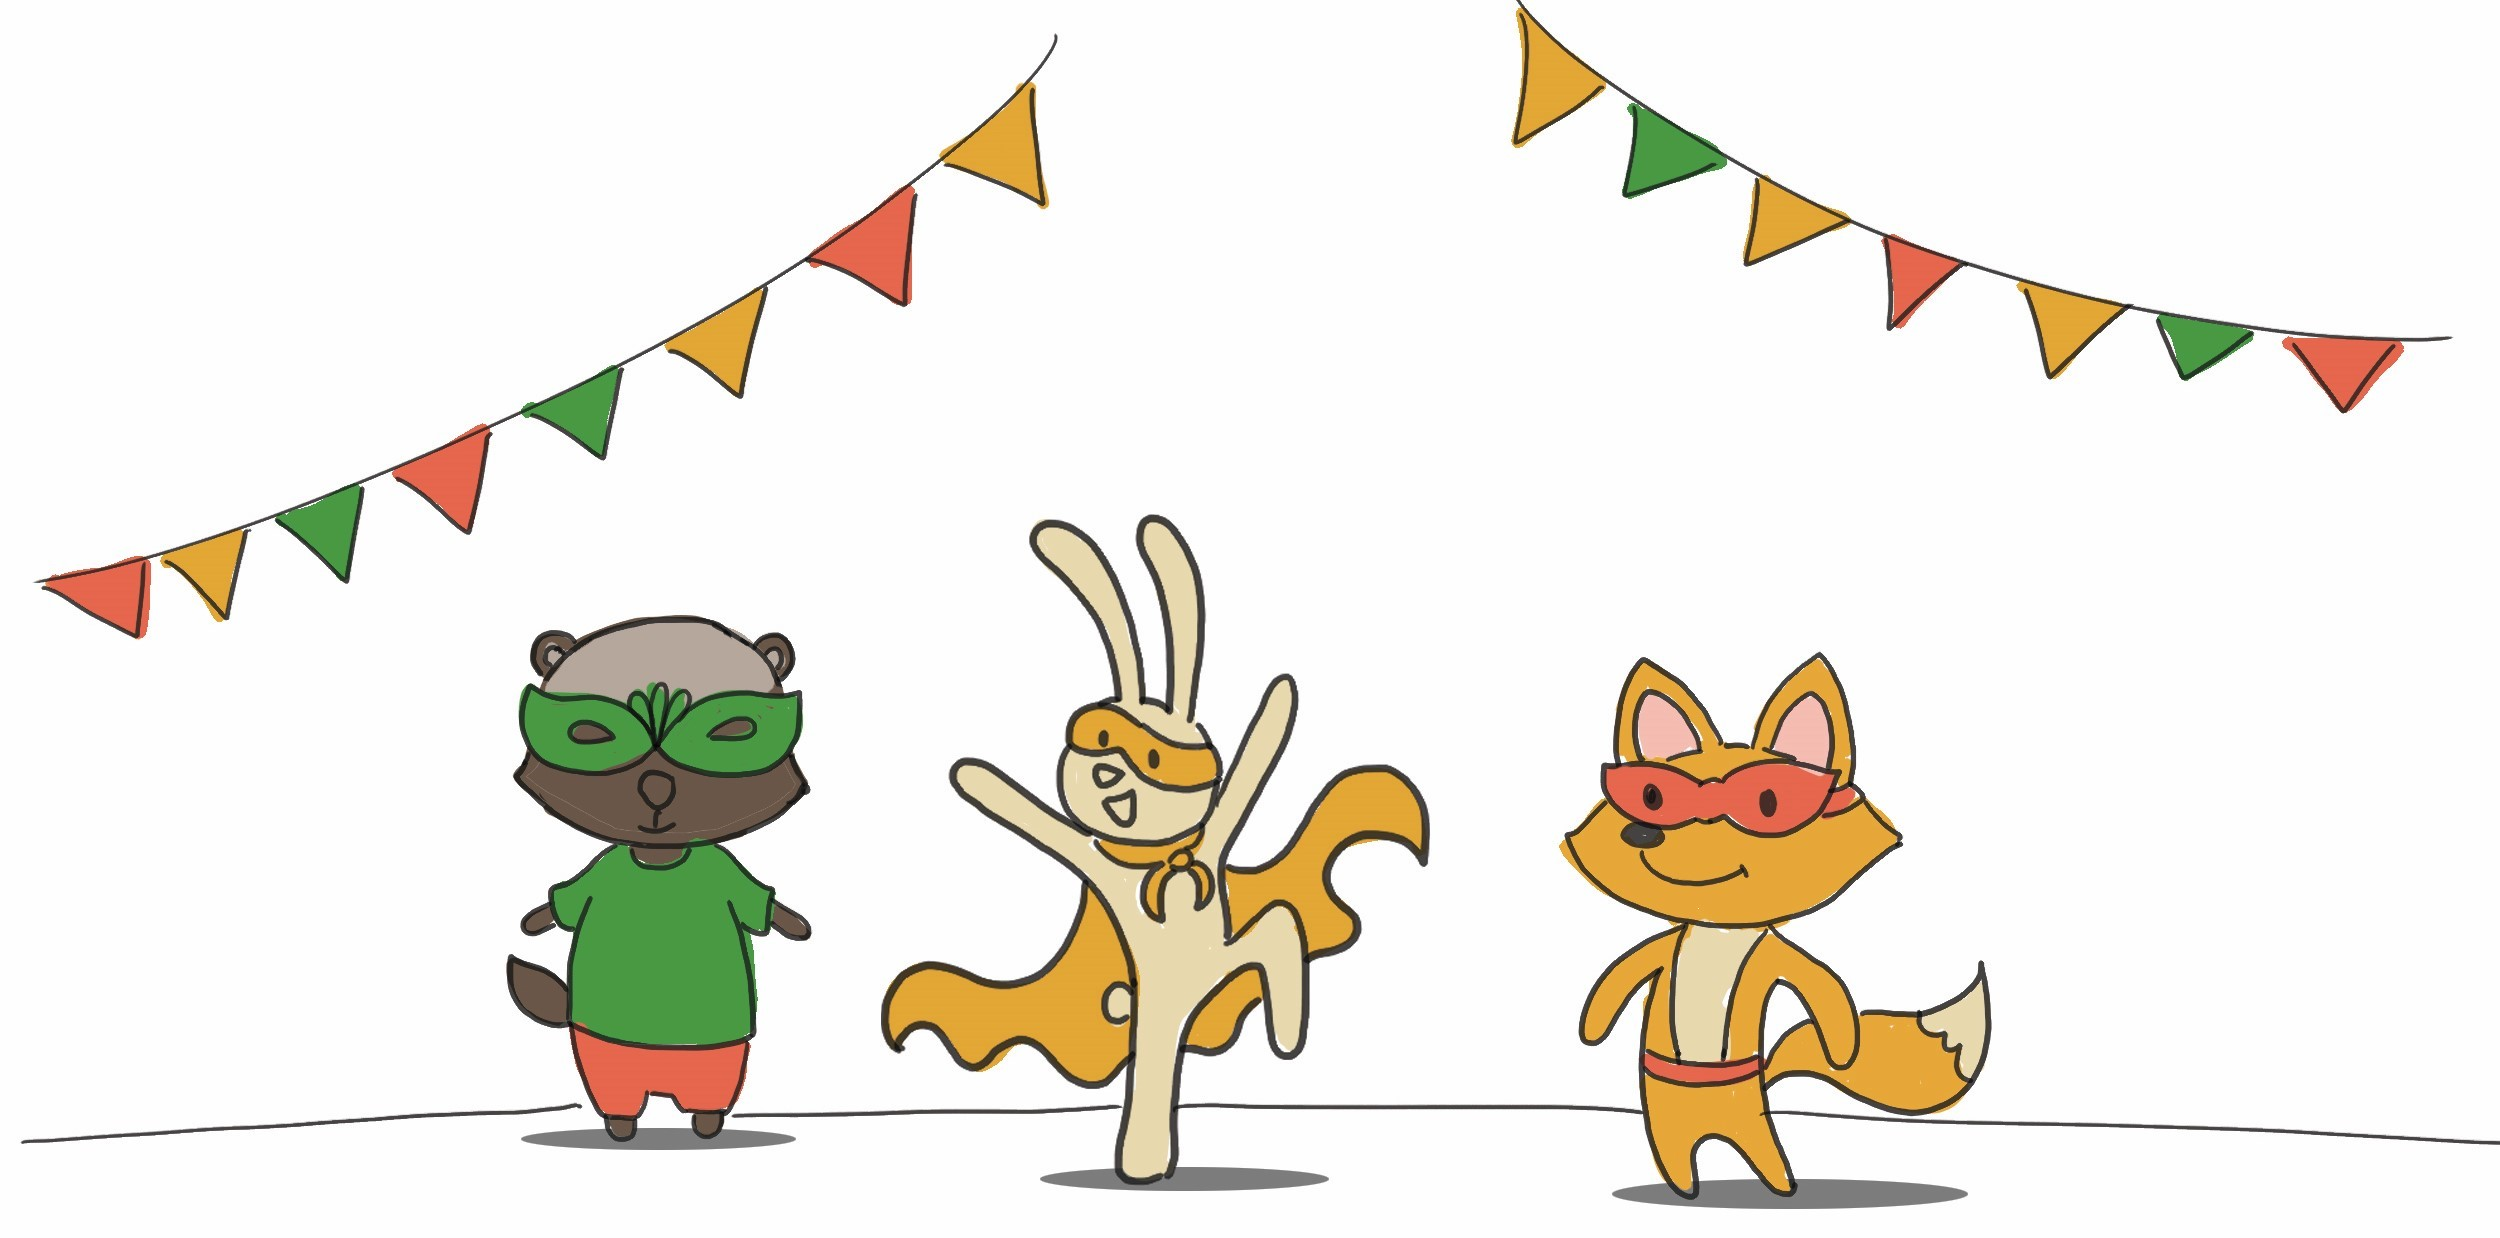
\includegraphics[width=1\linewidth]{Pi4_bai5}
		\vspace*{-20pt}
	\end{figure}
	Hai năm trước, có $12$ ``cáo" và $28$ ``sói" tại vũ hội, một năm trước -- có $15$ ``thỏ rừng", $10$ ``cáo" và $15$ ``lửng", và năm nay -- $15$ ``thỏ rừng" và $25$ ``cáo" . Hỏi loài thú nào có nhiều nhất trong rừng? 
	\vskip 0.1cm
	\textit{Lời giải.} Các em hãy viết dữ kiện của bài toán dưới dạng bảng.
	\begin{table}[H]
		\renewcommand{\arraystretch}{1.2}
		\resizebox{\columnwidth}{!}{\begin{tabular}{|l|c|c|c|c|}
			\hline
			&\makecell{Hai năm\\ trước}&\makecell{Một năm\\ trước}&Năm nay\\
			\hline
			Sói	&$28$& & \\
			\hline
			Cáo &$12$&$10$ &$25$ \\
			\hline
			Thỏ rừng& & $15$&$15$\\
			\hline
			Lửng& & $15$&\\
			\hline
		\end{tabular}}
	\end{table}
	Hãy nhìn vào những con ``thỏ rừng". Trong hai năm qua đã có $30$ con vật đeo mặt nạ ``thỏ rừng". Tất cả đều là những con vật khác nhau, vì sẽ không con nào đeo mặt nạ ``thỏ rừng" trong hai năm liên tiếp. Và tất nhiên đó cũng không phải là thỏ. Điều này có nghĩa là có ít nhất $30$ con không phải thỏ rừng trong rừng, tức là không quá $40 - 30 = 10$ (con thỏ rừng). Lập luận tương tự về những con vật đeo mặt nạ ``cáo" tại lễ hội trong hai năm qua cho thấy rằng trong rừng có không quá $40 - 10 - 25 = 5$ (con cáo). Hai năm trước, có $28$ ``con sói" tại lễ hội hóa trang, và tất cả những con này không phải là sói thật, do đó không có hơn $40 - 28 = 12$ (con sói). Vậy, sói, cáo và thỏ rừng cộng lại không quá $12 + 5 + 10 = 27$ (con). Điều này có nghĩa là có ít nhất $40 - 27 = 13$ (con lửng), và đây là loài động vật có số lượng nhiều nhất trong rừng.
	\vskip 0.1cm
	Lưu ý rằng có thể chọn số lượng động vật của mỗi loài và phân phát mặt nạ sao cho đáp ứng tất cả các điều kiện của bài toán.
	\vskip 0.1cm
	$\pmb{6.}$ $a)$	Có tám bạn học sinh giải một đề thi gồm $8$ bài toán. Khi tổng kết lại, cô giáo thấy rằng với mỗi bài toán lại có đúng  năm bạn học sinh giải được bài đó. Chứng minh rằng có hai học sinh sao cho với mỗi bài toán trong đề có ít nhất một trong hai em giải được.
	\vskip 0.1cm
	$b)$	Em hãy chỉ ra một ví dụ rằng, nếu với mỗi bài toán đều có đúng bốn bạn học sinh giải được, thì điều khẳng định ở câu $a)$ không đúng.
	\begin{figure}[H]
		\centering
		\vspace*{-10pt}
		\captionsetup{labelformat= empty, justification=centering}
		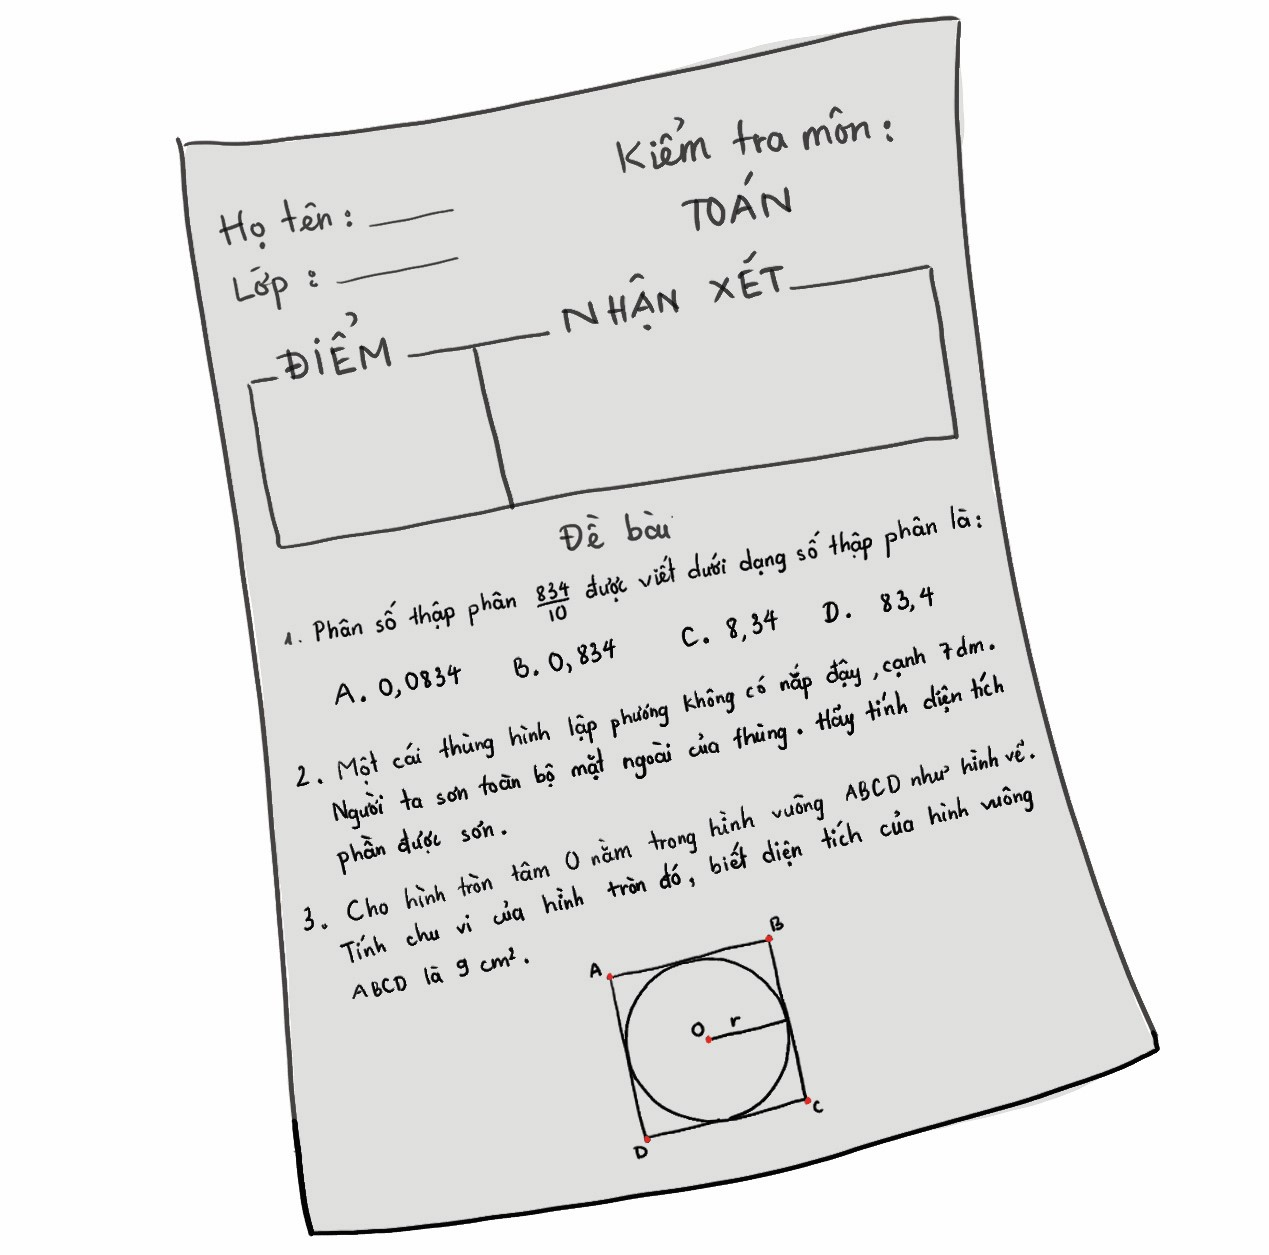
\includegraphics[width=0.7\linewidth]{Pi4_bai6}
		\vspace*{-5pt}
	\end{figure}
	\textit{Lời giải.} 	$a)$ Ta sẽ gọi một bộ ba gồm hai học sinh và một bài toán mà cả hai em đều không giải được là \textit{được đánh dấu}. Vì mỗi bài toán không giải được bởi đúng ba học sinh nên mỗi bài toán tương ứng với ba bộ ba \textit{được đánh dấu}. Vì vậy, có tổng cộng $24$ bộ ba như vậy. Mặt khác, có $7 \times 8 : 2 = 28$ cặp học sinh. Do đó, có một cặp học sinh không thuộc bất kỳ bộ ba nào \textit{được đánh dấu}. Điều này có nghĩa là hai em trong cặp này đã giải được tất cả các bài trong đề.
	\vskip 0.1cm
	$b)$ Ta có thể đưa ra một ví dụ như bảng sau mà mỗi bài toán được giải bởi đúng $4$ học sinh và không có cặp học sinh nào giải được mọi bài toán.
	\begin{table}[H]
		\renewcommand{\arraystretch}{1.2}
		\resizebox{\columnwidth}{!}{\begin{tabular}{|c|c|c|c|c|c|c|c|c|}
			\hline
			\multirow{2}{*}{Học sinh} & \multicolumn{8}{c|}{Bài toán}\\
			\cline{2-9}
			& $1$&$2$&$3$&$4$&$5$&$6$&$7$&$8$\\
			\hline
			$1$&$+$&$+$&$+$&$-$&$-$&$+$&$-$&$+$\\
			\hline
			$2$&$+$&$+$&$+$&$-$&$-$&$-$&$+$&$+$\\
			\hline
			$3$&$+$&$+$&$-$&$+$&$-$&$-$&$+$&$+$\\
			\hline
			$4$&$+$&$-$&$-$&$+$&$+$&$-$&$+$&$-$\\
			\hline
			$5$&$-$&$+$&$+$&$+$&$+$&$-$&$-$&$+$\\
			\hline
			$6$&$-$&$-$&$+$&$+$&$-$&$+$&$+$&$-$\\
			\hline
			$7$&$-$&$-$&$-$&$-$&$+$&$+$&$-$&$-$\\
			\hline
			$8$&$-$&$-$&$-$&$-$&$+$&$+$&$-$&$-$\\
			\hline
		\end{tabular}}
	\end{table}
\end{multicols}
\newpage
\blfootnote{$^1$\color{toancuabi}Trường Liên cấp Hội nhập Quốc tế iSchool Quảng Trị.}
\begingroup  
\AddToShipoutPicture*{\put(116,650){
\includegraphics[scale=1]{../tieude10.pdf}}}  
\centering
\endgroup
\vspace*{55pt} 

\begin{multicols}{2}
	\textbf{\color{toancuabi}Gấp trái tim bằng giấy}
	\vskip 0.1cm
	Các em chỉ cần chuẩn bị một tờ giấy màu hình vuông. Sau đó hãy làm theo các bước chỉ dẫn như sau là đã có được một trái tim xinh xắn bằng giấy rồi!
	\vskip 0.1cm
	\textit{Bước} $1$: Gấp đôi tờ giấy hình vuông $2$ lần để tạo nếp. 
	\begin{figure}[H]
			\vspace*{-5pt}
			\centering
			\captionsetup{labelformat= empty, justification=centering}
			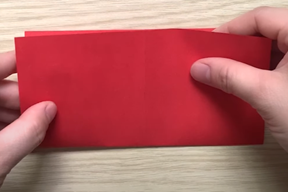
\includegraphics[height= 0.327\linewidth]{20}
			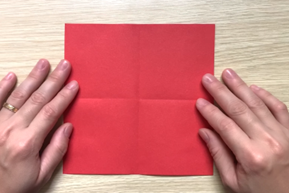
\includegraphics[height= 0.327\linewidth]{21}
			\vspace*{-10pt}
		\end{figure}
	\textit{Bước} $2$: Gấp $\dfrac{1}{4}$ tờ giấy lên phía trên chạm vào chính giữa tờ giấy. Dùng tay miết nhẹ để tạo nếp gấp.
	\begin{figure}[H]
			\vspace*{-5pt}
			\centering
			\captionsetup{labelformat= empty, justification=centering}
			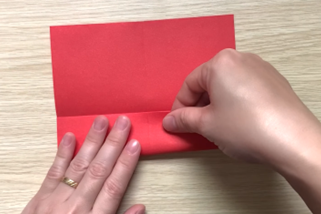
\includegraphics[width= 1\linewidth]{22}
			\vspace*{-15pt}
		\end{figure}
	Bước $3$: Lật mặt sau tờ giấy lại rồi gấp như các hình minh họa bên dưới. 
	\begin{figure}[H]
			\vspace*{-5pt}
			\centering
			\captionsetup{labelformat= empty, justification=centering}
			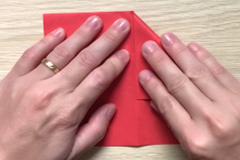
\includegraphics[height= 0.327\linewidth]{23}
			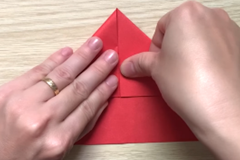
\includegraphics[height= 0.327\linewidth]{24}
			\vspace*{-15pt}
		\end{figure}
		\begin{figure}[H]
			\vspace*{5pt}
			\centering
			\captionsetup{labelformat= empty, justification=centering}
			
\includegraphics[width=1\linewidth]{25}
			\vspace*{-15pt}
		\end{figure}
	\textit{Bước} $4$: Tiếp tục lật mặt sau tờ giấy lại rồi gấp như hình minh họa. 
	\begin{figure}[H]
			\vspace*{-5pt}
			\centering
			\captionsetup{labelformat= empty, justification=centering}
			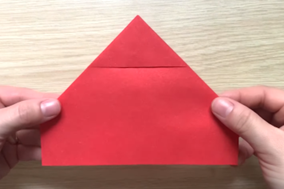
\includegraphics[height= 0.327\linewidth]{26}
			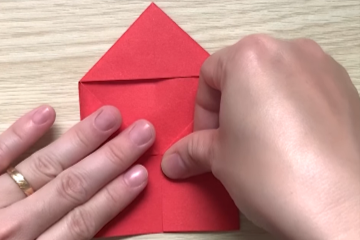
\includegraphics[height= 0.327\linewidth]{27}
			
			\vspace*{1pt}
			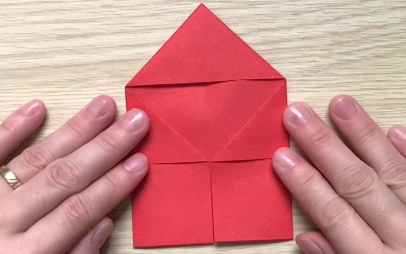
\includegraphics[width=1\linewidth]{28}
			\vspace*{-10pt}
		\end{figure}
	\textit{Bước} $5$: Gấp hai góc phía dưới lên.
	\begin{figure}[H]
			\vspace*{-5pt}
			\centering
			\captionsetup{labelformat= empty, justification=centering}
			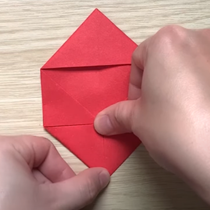
\includegraphics[height= 0.485\linewidth]{29}
			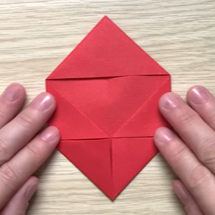
\includegraphics[height= 0.485\linewidth]{30}
			\vspace*{-10pt}
		\end{figure}
	\textit{Bước} $6$: Gấp đôi hình lại sao cho phần nhọn của tam giác phía dưới trùng khớp với phần nhọn của tam giác phía trên. Dùng tay miết nhẹ để tạo nếp gấp rồi mở ra.
	\begin{figure}[H]
			\vspace*{-5pt}
			\centering
			\captionsetup{labelformat= empty, justification=centering}
			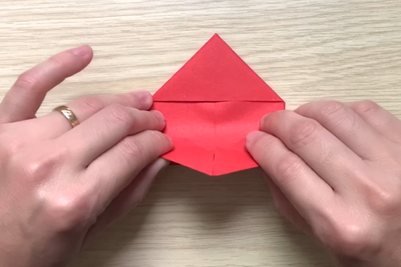
\includegraphics[height=0.327\linewidth]{31}
			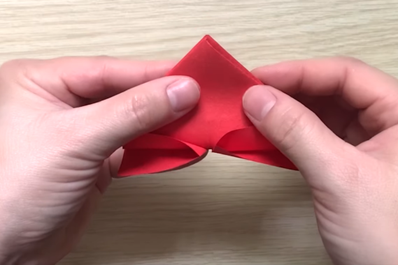
\includegraphics[height=0.327\linewidth]{32}
%			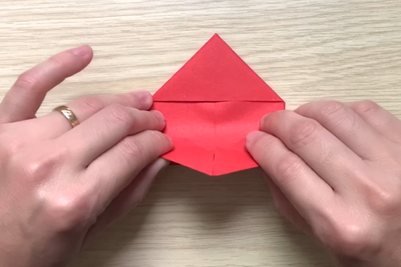
\includegraphics[width= 1\linewidth]{31}
%			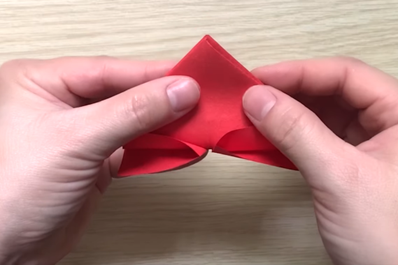
\includegraphics[width= 1\linewidth]{32}
			\vspace*{-15pt}
		\end{figure}
	\textit{Bước} $7$: Luồn phần nhọn của tam giác phía dưới vào kẽ hở của tam giác phía trên.
	\begin{figure}[H]
			\vspace*{-5pt}
			\centering
			\captionsetup{labelformat= empty, justification=centering}
			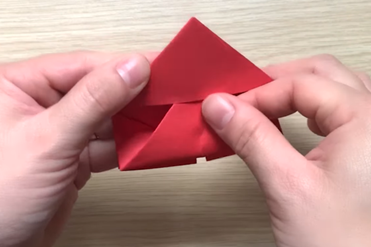
\includegraphics[height=0.327\linewidth]{33}
			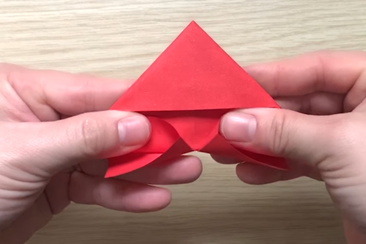
\includegraphics[height=0.327\linewidth]{34}
%			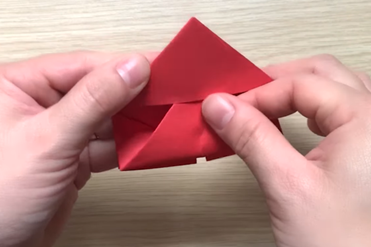
\includegraphics[width= 1\linewidth]{33}
%			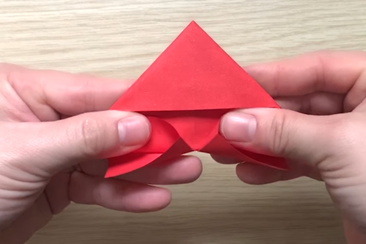
\includegraphics[width= 1\linewidth]{34}
			\vspace*{-15pt}
		\end{figure}
	\textit{Bước} $8$: Gấp hai góc nhỏ như hình minh họa.
		\begin{figure}[H]
			\vspace*{-5pt}
			\centering
			\captionsetup{labelformat= empty, justification=centering}
			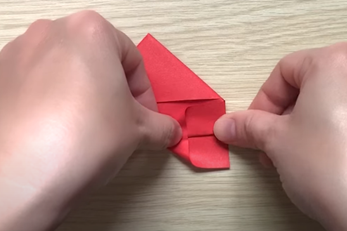
\includegraphics[height= 0.327\linewidth]{35}
			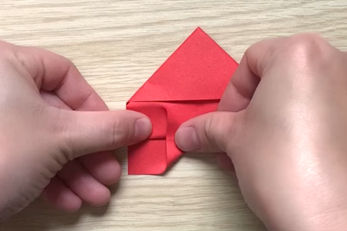
\includegraphics[height= 0.327\linewidth]{36}
			
			\vspace*{1pt}
			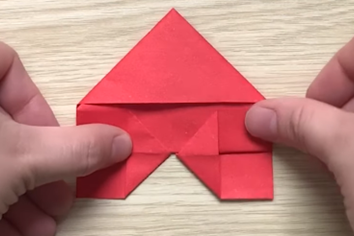
\includegraphics[height= 0.327\linewidth]{37}
			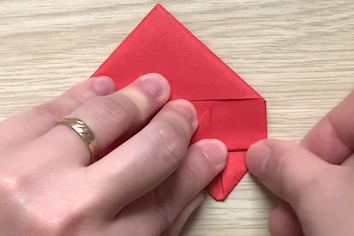
\includegraphics[height= 0.327\linewidth]{38}
			
			\vspace*{1pt}
			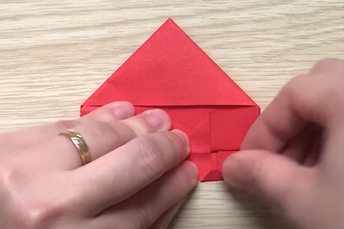
\includegraphics[height= 0.327\linewidth]{39}
			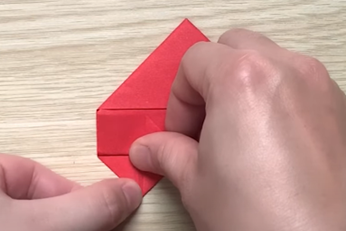
\includegraphics[height= 0.327\linewidth]{40}
			
			\vspace*{1pt}
			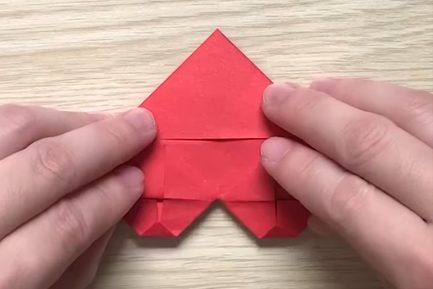
\includegraphics[height= 0.327\linewidth]{41}
			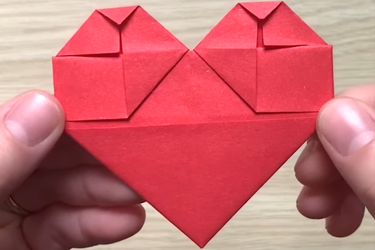
\includegraphics[height= 0.327\linewidth]{42}
%			\vspace*{-10pt}
		\end{figure}
		\begin{figure}[H]
			\vspace*{5pt}
			\centering
			\captionsetup{labelformat= empty, justification=centering}
			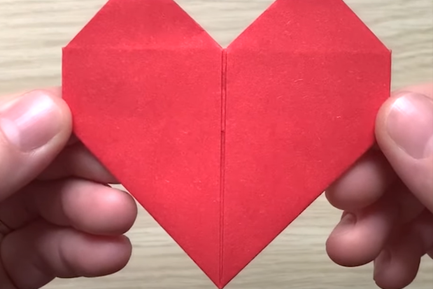
\includegraphics[width= 1\linewidth]{43}
			\vspace*{-10pt}
		\end{figure}
	Như vậy là chúng ta đã hoàn thành xong việc gấp trái tim bằng giấy rồi. Trái tim bằng giấy em vừa gấp xong có bao nhiêu trục đối xứng vậy?
	\begin{figure}[H]
			\vspace*{-5pt}
			\centering
			\captionsetup{labelformat= empty, justification=centering}
			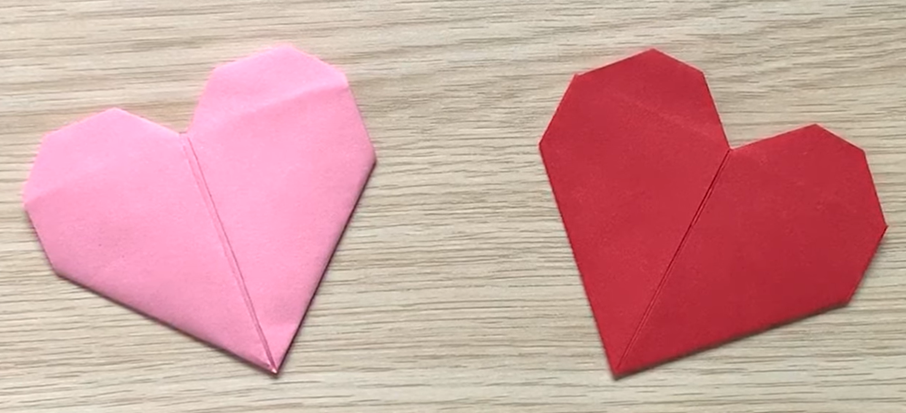
\includegraphics[width= 1\linewidth]{44}
			\vspace*{-15pt}
		\end{figure}
	\textbf{\color{toancuabi}Tài liệu tham khảo}
	\vskip 0.1cm
	[$1$] \url{https://www.youtube.com/watch?v=MUdeSi-dHGY}
	\vskip 0.1cm
	[$2$] \url{https://www.youtube.com/watch?v=paEAVS_9UwY}
	\vskip 0.1cm
	[$3$] \url{https://thuthuatchoi.com/huong-dan-c}\\
	\url{ach-choi-day-ayatori-cac-hinh-khac-nhau.html}
\end{multicols}
\newpage
\begingroup
\thispagestyle{toancuabinone}
\blfootnote{$^1$\color{toancuabi}Ottawa, Canada.}
\AddToShipoutPicture*{\put(60,733){
\includegraphics[width=17.2cm]{../mathc.pdf}}}
%\AddToShipoutPicture*{\put(-2,733){
\includegraphics[width=17.2cm]{../mathl.pdf}}} 
\AddToShipoutPicture*{\put(140,675){\includegraphics[scale=1]{../tieude6.pdf}}} 
\centering
\endgroup
\graphicspath{{../toancuabi/pic/}}
\vspace*{33pt}

\begin{multicols}{2}
	In this article, we discuss a few games and principles associated with solutions to the problems posed by the games.
	\vskip 0.2cm
	\PIbox{{\color{toancuabi}\textbf{Example} (Pigeonhole Principle)\textbf{.}}
		Each square of a $3 \times 3$ board is filled with one of the numbers $-1, 0, +1$. See the figure below for an example.
		Viet calculates the sums of the rows, columns, and two main diagonals. He found that there are at least two equal sums.
		For example, in the example below, both the sums of the second and third rows are $0$.
		Is it always true that there are at least two equal sums?}
	\vskip 0.1cm
	\begin{figure}[H]
		\vspace*{-5pt}
		\centering
		\captionsetup{labelformat= empty, justification=centering}
		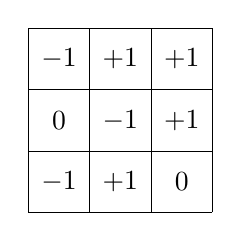
\begin{tikzpicture}[scale=0.78]
			\draw (0,0) grid (3,3);
			\draw (0.5,0.5) node {$-1$};
			\draw (1.5,0.5) node {$+1$};
			\draw (2.5,0.5) node {$0$};
			\draw (0.5,1.5) node {$0$};
			\draw (1.5,1.5) node {$-1$};
			\draw (2.5,1.5) node {$+1$};
			\draw (0.5,2.5) node {$-1$};
			\draw (1.5,2.5) node {$+1$};
			\draw (2.5,2.5) node {$+1$};
		\end{tikzpicture}
		\vspace*{-10pt}
	\end{figure}
	\textit{Solution.}
	The answer is yes. The largest possible sum is $3$ and the smallest is $-3.$
	There are $7$ possible values $-3,-2,...,2,3$ for $8$ sums, so two of the sums must be equal to each other.
	\vskip 0.1cm	
	In this example, we have applied the Pigeonhole Principle: \textit{if $n+1$ or more pigeons are placed in $n$ holes, then one hole must contain two or more pigeons.} 
	\vskip 0.2cm
	\PIbox{{\color{toancuabi}\textbf{Example} (Nothing ever changes)\textbf{.}}
		Each square of the  board contains a $+$ or $-$ signs, see the board the left,
		which contains a single $-$ at the square intersection of the first row and second column.}
	\vskip 0.1cm
	\vspace*{0.1pt}
	\vspace*{-8pt}
	\PIbox{
		At each step, you can change all the signs in a row, a column, or a diagonal to their opposite ones, i.e. $+$ to $-$, and $-$  to $+$.
		An example of how a column is changed shown as below in the board on the right.}
	\begin{center}
		\begin{tikzpicture}[scale=0.78]
			\draw [fill=cackithi!50] (1,0) rectangle (2,4);
			\draw [fill=cackithi!50] (6,0) rectangle (7,4);
			\draw (0,0) grid (4,4);
			\draw (0.5,0.5) node {$+$};
			\draw (1.5,0.5) node {$+$};
			\draw (2.5,0.5) node {$+$};
			\draw (3.5,0.5) node {$+$};
			\draw (0.5,1.5) node {$+$};
			\draw (1.5,1.5) node {$+$};
			\draw (2.5,1.5) node {$+$};
			\draw (3.5,1.5) node {$+$};
			\draw (0.5,2.5) node {$+$};
			\draw (1.5,2.5) node {$+$};
			\draw (2.5,2.5) node {$+$};
			\draw (3.5,2.5) node {$+$};
			\draw (0.5,3.5) node {$+$};
			\draw (1.5,3.5) node {$-$};
			\draw (2.5,3.5) node {$+$};
			\draw (3.5,3.5) node {$+$};
			\draw (5,0) grid (9,4);
			\draw (5.5,0.5) node {$+$};
			\draw (6.5,0.5) node {$-$};
			\draw (7.5,0.5) node {$+$};
			\draw (8.5,0.5) node {$+$};
			\draw (5.5,1.5) node {$+$};
			\draw (6.5,1.5) node {$-$};
			\draw (7.5,1.5) node {$+$};
			\draw (8.5,1.5) node {$+$};
			\draw (5.5,2.5) node {$+$};
			\draw (6.5,2.5) node {$-$};
			\draw (7.5,2.5) node {$+$};
			\draw (8.5,2.5) node {$+$};
			\draw (5.5,3.5) node {$+$};
			\draw (6.5,3.5) node {$+$};
			\draw (7.5,3.5) node {$+$};
			\draw (8.5,3.5) node {$+$};
		\end{tikzpicture}
	\end{center}
	\textit{Solution.}
	Take a look at the squares colored \textcolor{red!50}{red}.
	\begin{center}
		\begin{tikzpicture}[scale=0.78]
			\draw [fill=cackithi!50] (1,0) rectangle (2,4);
			\draw [fill=cackithi!50] (6,0) rectangle (7,4);
			\draw [fill=red!50] (0,1) rectangle (1,3);
			\draw [fill=red!50] (1,3) rectangle (3,4);
			\draw [fill=red!50] (3,3) rectangle (4,1);
			\draw [fill=red!50] (3,1) rectangle (1,0);
			\draw (0,0) grid (4,4);
			\draw (0.5,0.5) node {$+1$};
			\draw (1.5,0.5) node {$+1$};
			\draw (2.5,0.5) node {$+1$};
			\draw (3.5,0.5) node {$+1$};
			\draw (0.5,1.5) node {$+1$};
			\draw (1.5,1.5) node {$+1$};
			\draw (2.5,1.5) node {$+1$};
			\draw (3.5,1.5) node {$+1$};
			\draw (0.5,2.5) node {$+1$};
			\draw (1.5,2.5) node {$+1$};
			\draw (2.5,2.5) node {$+1$};
			\draw (3.5,2.5) node {$+1$};
			\draw (0.5,3.5) node {$+1$};
			\draw (1.5,3.5) node {$-1$};
			\draw (2.5,3.5) node {$+1$};
			\draw (3.5,3.5) node {$+1$};
			\draw (5,0) grid (9,4);
			\draw (5.5,0.5) node {$+1$};
			\draw (6.5,0.5) node {$-1$};
			\draw (7.5,0.5) node {$+1$};
			\draw (8.5,0.5) node {$+1$};
			\draw (5.5,1.5) node {$+1$};
			\draw (6.5,1.5) node {$-1$};
			\draw (7.5,1.5) node {$+1$};
			\draw (8.5,1.5) node {$+1$};
			\draw (5.5,2.5) node {$+1$};
			\draw (6.5,2.5) node {$-1$};
			\draw (7.5,2.5) node {$+1$};
			\draw (8.5,2.5) node {$+1$};
			\draw (5.5,3.5) node {$+1$};
			\draw (6.5,3.5) node {$+1$};
			\draw (7.5,3.5) node {$+$};
			\draw (8.5,3.5) node {$+1$};
		\end{tikzpicture}
	\end{center}	
	If we replace the $+$ sign by $+1$ and the $-$ sign by $-1$, then at the beginning the product of all numbers in these red square is $-1.$ 
	Easy to see that each operation to change all the signs in a row, a column or a diagonal shall change exactly two red squares.
	Whatever the numbers in the two red squares, the product of their negates remain same.
	Since the product of the red squares at the beginning is $-1,$ so it cannot be changed at all.
	\vskip 0.1cm
	In this example, we have applied the Invariant Principle: \textit{In mathematics, an invariant is a property of a mathematical object
		(or a class of mathematical objects) which remains unchanged after operations or transformations of a certain type are applied to the objects.} 
	\vskip 0.2cm
	\PIbox{{\color{toancuabi}\textbf{Example} (Integers are well--ordered)\textbf{.}}
		On a stormy night, ten students from the \textit{Math, Chess, and Coding Club in Ottawa} went to a party.
		They left their shoes in the foyer in order to keep the carpet clean. After the dinner, there was a power outage.
		So the students, leaving one by one, put on, at random, any pair of shoes big enough for their feet (each pair of shoes stay together).
		Any student who couldn't find a pair of shoes big enough spent the night at the place of the party.
		\vskip 0.1cm	
		What is the largest number of students who would have to spend the night? Show an example for this number.
		\textit{Note that no two students wear the same size shoes.}}
	\vskip 0.2cm
	\textit{Solution.}
	It is easy to see that if the five students with smallest feet left first wearing all five largest pairs of shoes
	then none of the remaining student can find a pair of shoes to leave.
	Now let us assume that there were $6$ students who would have to spend the night. In that case, there would be $6$ pairs of shoes left. It is immediate to see that one of those $6$ pair of shoes would belong to one of the $6$ students. This is a contradiction and so the assumed situation could not happen.
	\vskip 0.1cm
	In this example, we have applied the \textit{Well--Ordering Principle: the positive integers are well--ordered.
		An ordered set is said to be well--ordered if each and every nonempty subset has a least element in this ordering.} 
	\vskip 0.2cm
	\PIbox{{\color{toancuabi}\textbf{Example} (Invariant to reach end--state with desired outcomes)\textbf{.}}
		In a darkroom there are two tables. The first one is empty and the second one is covered by a layer of nickels
		(one nickel thick, so no coin is on top of another), in which $31$ coins are tails up and the rest are heads up.}
	\vskip 0.1cm
	\PIbox{
		Minh enters the room with the task of transferring some coins from the second table to the first table
		(he wears gloves, so he cannot feel the faces of the coins). He can flip over any number of coins when transferring them.
		\vskip 0.1cm
		Is it possible that when he leaves the room, the numbers of nickles are the same on both tables?}
	\vskip 0.2cm
	\textit{Solution.}
	If Minh turns a coin on the second table during transfer to the first one,
	then the number of coins \textit{tails--up} on the second table will be reduced by one if it was a \textit{tails--up} coin,
	or the number of coins \textit{tails--up} on the first table is increased by one if it was a \textit{heads--up} coin.
	In any case, the difference between the \textit{tails--up} coins on the second and first tables will be reduced by one
	(this is an \textit{invariant}.) Hence, after $31$ moves, they will be the same.
	\vskip 0.1cm
	In this example, we have applied the \textit{Invariant Principle} with a twist.
	Note that in every turn the difference between the \textit{tails--up} coins on the second and first tables will be reduced by one,
	since at the beginning, in other words, at the \textit{start state} this difference is $31,$
	thus after $31$ turns the game reaches the \textit{end--state} where the difference is $0.$
	\vskip 0.2cm
	\PIbox{{\color{toancuabi}\textbf{Example} (Winning positions)\textbf{.}}
		In a two--player game, Berry and Cherry take turns removing marbles a pile as follows:
		\vskip 0.1cm
		$\bullet$ Berry always goes from first.
		\vskip 0.1cm
		$\bullet$ In his or her turn, the player must remove exactly $2$, $4$ or $5$ marbles from the pile.
		\vskip 0.1cm
		$\bullet$ The player who at some point is unable to make a move (in other words, the player cannot remove $2$, $4$ or $5$ marbles from the pile) loses the game.
		\vskip 0.1cm
		They play $14$ games with $\{8, 9, \ldots, 21\}$ as the initial number of marbles in the pile.
		What games does Cherry always win, regardless of what Berry does?}
	\vskip 0.2cm
	\textit{Solution.}
	The positive integers from $0$ to $21$ can be divided into 7 groups of numbers based on their remainders when divided by $7$,
	\begin{align*}
		&G_0=\{0,7,14,21\}, &&G_1=\{1,8,15\},\\
		& G_2=\{2,9,16\}, &&G_3=\{3,10,17\},\\
		& G_4=\{4,11,18\},&&G_5=\{5,12,19\},\\
		& G_6=\{6,13,20\}
	\end{align*}
	It is easy to verify the following claim:
	\vskip 0.2cm
	\PIbox{\textbf{\color{toancuabi}Claim.}
		If $n$ is a number in $G_0$ and $G_1$ then $n-2$, $n-4$, and $n-5$ are in $G_2,G_3,G_4,G_5,$ or $G_6$.}
	\vskip 0.2cm
	Now, by the rules of the game, it is obvious that $\{0, 1\}$ are \textit{losing} positions and $\{2,4,5\}$ are \textit{winning} positions.
	Furthermore, because $3-2=6-5=1$, so $\{3,6\}$ are also \textit{winning} positions, too.
	\vskip 0.1cm
	Therefore $G_0$ and $G_1$ contain all \textit{losing} positions, while $G_2,G_3,G_4,G_5,$ and $G_6$ containing all \textit{winning} positions.
	A player, who is in a \textit{winning} position, can always force the game into a \textit{losing} position.
	Thus, Cherry will win the game if the game starts with a \textit{losing} position.
	Thus, the games that Cherry wins are $\{8,14,15,21\}$.
	\vskip 0.2cm
	\PIbox{
	\centerline{\textbf{\color{toancuabi}Vocabulary}}
	\vskip 0.2cm
	{\color{toancuabi}principle (n):} nguyên lý
	\vskip 0.1cm
	{\color{toancuabi}Pigeonhole Principle (n):} Nguyên lý chuồng bồ câu 
	\vskip 0.1cm
	{\color{toancuabi}Invariant Principle (n):} Nguyên lý bất biến
	\vskip 0.1cm
	{\color{toancuabi}Well--ordering Principle (n):} Nguyên lý sắp thứ tự tốt
	\vskip 0.1cm
	{\color{toancuabi}operation (n):} phép toán
	\vskip 0.1cm
	{\color{toancuabi}transformation (n):} phép biến đổi
	\vskip 0.1cm
	{\color{toancuabi}foyer (n):} tiền sảnh (của một tòa nhà lớn)
	\vskip 0.1cm
	{\color{toancuabi}power outage (n):} cúp điện
	\vskip 0.1cm
	{\color{toancuabi}take turns (v):} thay phiên nhau
	\vskip 0.1cm
	{\color{toancuabi}marble (n):} viên đá
	\vskip 0.1cm
	{\color{toancuabi}pile (n):} chồng, đống
	\vskip 0.1cm
	{\color{toancuabi}claim (n):} nhận định
	\vskip 0.1cm
	{\color{toancuabi}remainder (n):} số dư
	\vskip 0.1cm
	{\color{toancuabi}start state (n):} trạng thái bắt đầu
	\vskip 0.1cm
	{\color{toancuabi}end state (n):} trạng thái kết thúc
	\vskip 0.1cm
	{\color{toancuabi}winning position (n):} vị trí thắng
	\vskip 0.1cm
	{\color{toancuabi}losing position (n):} vị trí thua}
\end{multicols}